\begin{enumerate}[label=\thechapter.\arabic*,ref=\thechapter.\theenumi]
	\item Given that a fair coin is marked 1 on one face and 6 on the other and a fair die are tossed. Find the probability that the sum turns up to be 3 and 12. 
		\\
		\solution
		\iffalse
\let\negmedspace\undefined 
 \let\negthickspace\undefined 
 \documentclass[journal,12pt,onecolumn]{IEEEtran} 
 %\documentclass[conference]{IEEEtran} 
 %\IEEEoverridecommandlockouts 
 % The preceding line is only needed to identify funding in the first footnote. If that is unneeded, please comment it out. 
 \usepackage{cite} 
 \usepackage{amsmath,amssymb,amsfonts,amsthm} 
 \usepackage{algorithmic} 
 \usepackage{graphicx} 
 \usepackage{textcomp} 
 \usepackage{xcolor} 
 \usepackage{txfonts} 
 \usepackage{listings} 
 \usepackage{enumitem} 
 \usepackage{mathtools} 
 \usepackage{gensymb} 
 \usepackage[breaklinks=true]{hyperref} 
 \usepackage{tkz-euclide} % loads  TikZ and tkz-base 
 \usepackage{listings} 
 \usepackage{caption}
 % 
 %\usepackage{setspace} 
 %\usepackage{gensymb} 
 %\doublespacing 
 %\singlespacing 
  
 %\usepackage{graphicx} 
 %\usepackage{amssymb} 
 %\usepackage{relsize} 
  %\usepackage[cmex10]{amsmath} 
 %\usepackage{amsthm} 
 %\interdisplaylinepenalty=2500 
 %\savesymbol{iint} 
 %\usepackage{txfonts} 
 %\restoresymbol{TXF}{iint} 
 %\usepackage{wasysym} 
 %\usepackage{amsthm} 
 %\usepackage{iithtlc} 
 %\usepackage{mathrsfs} 
 %\usepackage{txfonts} 
 %\usepackage{stfloats} 
 %\usepackage{bm} 
 %\usepackage{cite} 
 %\usepackage{cases} 
 %\usepackage{subfig} 
 %\usepackage{xtab} 
 %\usepackage{longtable} 
 %\usepackage{multirow} 
 %\usepackage{algorithm} 
 %\usepackage{algpseudocode} 
 %\usepackage{enumitem} 
 %\usepackage{mathtools} 
 %\usepackage{tikz} 
 %\usepackage{circuitikz} 
 %\usepackage{verbatim} 
 %\usepackage{tfrupee} 
 %\usepackage{stmaryrd} 
 %\usetkzobj{all} 
 %    \usepackage{color}                                            %% 
 %    \usepackage{array}                                            %% 
 %    \usepackage{longtable}                                        %% 
 %    \usepackage{calc}                                             %% 
 %    \usepackage{multirow}                                         %% 
 %    \usepackage{hhline}                                           %% 
 %    \usepackage{ifthen}                                           %% 
   %optionally (for landscape tables embedded in another document): %% 
 %    \usepackage{lscape}      
 %\usepackage{multicol} 
 %\usepackage{chngcntr} 
 %\usepackage{enumerate} 
  
 %\usepackage{wasysym} 
 %\newcounter{MYtempeqncnt} 
 \DeclareMathOperator*{\Res}{Res} 
 %\renewcommand{\baselinestretch}{2} 
 \renewcommand\thesection{\arabic{section}} 
 \renewcommand\thesubsection{\thesection.\arabic{subsection}} 
 \renewcommand\thesubsubsection{\thesubsection.\arabic{subsubsection}} 
  
 \renewcommand\thesectiondis{\arabic{section}} 
 \renewcommand\thesubsectiondis{\thesectiondis.\arabic{subsection}} 
 \renewcommand\thesubsubsectiondis{\thesubsectiondis.\arabic{subsubsection}} 
  
 % correct bad hyphenation here 
 \hyphenation{op-tical net-works semi-conduc-tor} 
 \def\inputGnumericTable{}                                 %% 
  
 \lstset{ 
 %language=C, 
 frame=single,  
 breaklines=true, 
 columns=fullflexible 
 } 
 %\lstset{ 
 %language=tex, 
 %frame=single,  
 %breaklines=true 
 %} 
  
 \begin{document} 
 % 
  
  
 \newtheorem{theorem}{Theorem}[section] 
 \newtheorem{problem}{Problem} 
 \newtheorem{proposition}{Proposition}[section] 
 \newtheorem{lemma}{Lemma}[section] 
 \newtheorem{corollary}[theorem]{Corollary} 
 \newtheorem{example}{Example}[section] 
 \newtheorem{definition}[problem]{Definition} 
 %\newtheorem{thm}{Theorem}[section]  
 %\newtheorem{defn}[thm]{Definition} 
 %\newtheorem{algorithm}{Algorithm}[section] 
 %\newtheorem{cor}{Corollary} 
 \newcommand{\BEQA}{\begin{eqnarray}} 
 \newcommand{\EEQA}{\end{eqnarray}} 
 \newcommand{\define}{\stackrel{\triangle}{=}} 
  
 \bibliographystyle{IEEEtran} 
 %\bibliographystyle{ieeetr} 
  
  
 \providecommand{\mbf}{\mathbf} 
 \providecommand{\pr}[1]{\ensuremath{\Pr\left(#1\right)}} 
 \providecommand{\qfunc}[1]{\ensuremath{Q\left(#1\right)}} 
 \providecommand{\sbrak}[1]{\ensuremath{{}\left[#1\right]}} 
 \providecommand{\lsbrak}[1]{\ensuremath{{}\left[#1\right.}} 
 \providecommand{\rsbrak}[1]{\ensuremath{{}\left.#1\right]}} 
 \providecommand{\brak}[1]{\ensuremath{\left(#1\right)}} 
 \providecommand{\lbrak}[1]{\ensuremath{\left(#1\right.}} 
 \providecommand{\rbrak}[1]{\ensuremath{\left.#1\right)}} 
 \providecommand{\cbrak}[1]{\ensuremath{\left\{#1\right\}}} 
 \providecommand{\lcbrak}[1]{\ensuremath{\left\{#1\right.}} 
 \providecommand{\rcbrak}[1]{\ensuremath{\left.#1\right\}}} 
 \theoremstyle{remark} 
 \newtheorem{rem}{Remark} 
 \newcommand{\sgn}{\mathop{\mathrm{sgn}}} 
 \providecommand{\abs}[1]{\left\vert#1\right\vert} 
 \providecommand{\res}[1]{\Res\displaylimits_{#1}}  
 \providecommand{\norm}[1]{\left\lVert#1\right\rVert} 
 %\providecommand{\norm}[1]{\lVert#1\rVert} 
 \providecommand{\mtx}[1]{\mathbf{#1}} 
 \providecommand{\mean}[1]{E\left[ #1 \right]} 
 \providecommand{\fourier}{\overset{\mathcal{F}}{ \rightleftharpoons}} 
 %\providecommand{\hilbert}{\overset{\mathcal{H}}{ \rightleftharpoons}} 
 \providecommand{\system}{\overset{\mathcal{H}}{ \longleftrightarrow}} 
         %\newcommand{\solution}[2]{\textbf{Solution:}{#1}} 
 \newcommand{\solution}{\noindent \textbf{Solution: }} 
 \newcommand{\cosec}{\,\text{cosec}\,} 
 \providecommand{\dec}[2]{\ensuremath{\overset{#1}{\underset{#2}{\gtrless}}}} 
 \newcommand{\myvec}[1]{\ensuremath{\begin{pmatrix}#1\end{pmatrix}}} 
 \newcommand{\mydet}[1]{\ensuremath{\begin{vmatrix}#1\end{vmatrix}}} 
 %\numberwithin{equation}{section} 
 %\numberwithin{equation}{subsection} 
 %\numberwithin{problem}{section} 
 %\numberwithin{definition}{section} 
 %\makeatletter 
 %\@addtoreset{figure}{problem} 
 %\makeatother 
  
 %\let\StandardTheFigure\thefigure 
 \let\vec\mathbf 
 %\renewcommand{\thefigure}{\theproblem.\arabic{figure}} 
 %\renewcommand{\thefigure}{\theproblem} 
 %\setlist[enumerate,1]{before=\renewcommand\theequation{\theenumi.\arabic{equation}} 
 %\counterwithin{equation}{enumi} 
  
  
 %\renewcommand{\theequation}{\arabic{subsection}.\arabic{equation}} 
  
 %\def\putbox#1#2#3{\makebox[0in][l]{\makebox[#1][l]{}\raisebox{\baselineskip}[0in][0in]{\raisebox{#2}[0in][0in]{#3}}}} 
 %     \def\rightbox#1{\makebox[0in][r]{#1}} 
 %     \def\centbox#1{\makebox[0in]{#1}} 
 %     \def\topbox#1{\raisebox{-\baselineskip}[0in][0in]{#1}} 
 %     \def\midbox#1{\raisebox{-0.5\baselineskip}[0in][0in]{#1}} 
  
 \vspace{3cm} 
  
 \title{ Assignment 1 
  
         \Large AI1110: Probability and Random Variables 
  
          INDIAN INSTITUTE OF TECHNOLOGY, HYDERABAD 
 } 
 \author{ LAHARI GUNTI 
          
         AI22BTECH11008 
 } 
  
 \maketitle 
  
 \bigskip 
 \renewcommand{\thefigure}{\theenumi} 
 \renewcommand{\thetable}{\theenumi} 
 \textbf{11.16.3.5}: 
 Given that a fair coin is marked 1 on one face and 6 on the other and a fair die are tossed.find the probability sum turns up to be 3 and 12 \\ 
 \textbf{Solution}: 
 \fi
         Let the random variables  $X, Y$ denote the toss of a coin and roll of a dice respectively.
	 Since, 
                        \begin{align}
                                M_X(z) &= \frac{z^{-1}}{2}\brak{1 + z^{-5}},
				\\
                                 M_Y(z) &
                                 =\frac{z^{-1}\brak{1-z^{-6}}}{6\brak{1-z^{-1}}},
				 \\
                        M_Z(z) &= \sbrak{\frac{z^{-1} + z^{-6}}{2}}\sbrak{\frac{z^{-1}\brak{1-z^{-6}}}{6\brak{1-z^{-1}}}} 
                                \end{align}
				yielding
			 \begin{align}
				 p_Z\brak{n} = \begin{cases} \frac{1}{12} &  2 \leqslant\: n < 7 , \\ \frac{1}{6} &  n = 7, \\ \frac{1}{12} &  8 \leqslant\: n < 13 \end{cases}
			 \end{align}
			 See \figref{fig:ncert/11/16/3/5/pmf}.  Thus,
	   \begin{align}
		   \pr{Z = 3} = \frac{1}{12},\,
		      \pr{Z = 12} = \frac{1}{12}
	      \end{align}
			 \begin{figure}[!ht]
				 \centering
				 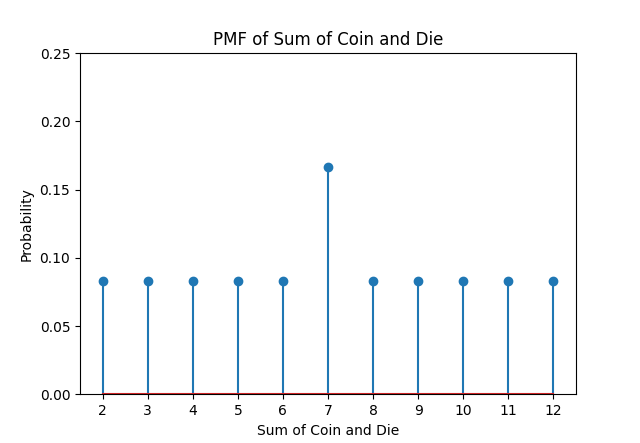
\includegraphics[width=\columnwidth]{ncert/11/16/3/5/figs/1.png}
				 \caption{pmf of the sum when coin and die are rolled simultaneously}
				 \label{fig:ncert/11/16/3/5/pmf}
			 \end{figure}

	\item A fair coin is tossed four times, and a person win Re 1 for each head and lose Rs 1.50 for each tail that turns up.
From the sample space calculate how many different amounts of money you can have after four tosses and the probability of having each of these amounts.\\
		\\
		\solution
		\iffalse
\let\negmedspace\undefined
\let\negthickspace\undefined
\documentclass[journal,12pt]{IEEEtran}

%\documentclass[conference]{IEEEtran}
%\IEEEoverridecommandlockouts
% The preceding line is only needed to identify funding in the first footnote. If that is unneeded, please comment it out.
\usepackage{cite}
\usepackage{amsmath,amssymb,amsfonts,amsthm}
\usepackage{algorithmic}
\usepackage{graphicx}
\usepackage{textcomp}
\usepackage{xcolor}
\usepackage{txfonts}
\usepackage{listings}
\usepackage{enumitem}
\usepackage{mathtools}
\usepackage{gensymb}
\usepackage[breaklinks=true]{hyperref}
\usepackage{tkz-euclide} % loads  TikZ and tkz-base
\usepackage{listings}
\usepackage{caption}
%
%\usepackage{setspace}
%\usepackage{gensymb}
%\doublespacing
%\singlespacing

%\usepackage{graphicx}
%\usepackage{amssymb}
%\usepackage{relsize}
%\usepackage[cmex10]{amsmath}
%\usepackage{amsthm}
%\interdisplaylinepenalty=2500
%\savesymbol{iint}
%\usepackage{txfonts}
%\restoresymbol{TXF}{iint}
%\usepackage{wasysym}
%\usepackage{amsthm}
%\usepackage{iithtlc}
%\usepackage{mathrsfs}
%\usepackage{txfonts}
%\usepackage{stfloats}
%\usepackage{bm}
%\usepackage{cite}
%\usepackage{cases}
%\usepackage{subfig}
%\usepackage{xtab}
%\usepackage{longtable}
%\usepackage{multirow}
%\usepackage{algorithm}
%\usepackage{algpseudocode}
%\usepackage{enumitem}
%\usepackage{mathtools}
%\usepackage{tikz}
%\usepackage{circuitikz}
%\usepackage{verbatim}
%\usepackage{tfrupee}
%\usepackage{stmaryrd}
%\usetkzobj{all}
%    \usepackage{color}                                            %%
%    \usepackage{array}                                            %%
%    \usepackage{longtable}                                        %%
%    \usepackage{calc}                                             %%
%    \usepackage{multirow}                                         %%
%    \usepackage{hhline}                                           %%
%    \usepackage{ifthen}                                           %%
  %optionally (for landscape tables embedded in another document): %%
%    \usepackage{lscape}     
%\usepackage{multicol}
%\usepackage{chngcntr}
%\usepackage{enumerate}

%\usepackage{wasysym}
%\newcounter{MYtempeqncnt}
\DeclareMathOperator*{\Res}{Res}
%\renewcommand{\baselinestretch}{2}
\renewcommand\thesection{\arabic{section}}
\renewcommand\thesubsection{\thesection.\arabic{subsection}}
\renewcommand\thesubsubsection{\thesubsection.\arabic{subsubsection}}

\renewcommand\thesectiondis{\arabic{section}}
\renewcommand\thesubsectiondis{\thesectiondis.\arabic{subsection}}
\renewcommand\thesubsubsectiondis{\thesubsectiondis.\arabic{subsubsection}}

% correct bad hyphenation here
\hyphenation{op-tical net-works semi-conduc-tor}
\def\inputGnumericTable{}                                 %%

\lstset{
%language=C,
frame=single, 
breaklines=true,
columns=fullflexible
}
%\lstset{
%language=tex,
%frame=single, 
%breaklines=true
%}

\begin{document}
%


\newtheorem{theorem}{Theorem}[section]
\newtheorem{problem}{Problem}
\newtheorem{proposition}{Proposition}[section]
\newtheorem{lemma}{Lemma}[section]
\newtheorem{corollary}[theorem]{Corollary}
\newtheorem{example}{Example}[section]
\newtheorem{definition}[problem]{Definition}
%\newtheorem{thm}{Theorem}[section] 
%\newtheorem{defn}[thm]{Definition}
%\newtheorem{algorithm}{Algorithm}[section]
%\newtheorem{cor}{Corollary}
\newcommand{\BEQA}{\begin{eqnarray}}
\newcommand{\EEQA}{\end{eqnarray}}
\newcommand{\define}{\stackrel{\triangle}{=}}
\newcommand\tab[1][1cm]{\hspace*{#1}}

\bibliographystyle{IEEEtran}
%\bibliographystyle{ieeetr}


\providecommand{\mbf}{\mathbf}
\providecommand{\pr}[1]{\ensuremath{\Pr\left(#1\right)}}
\providecommand{\qfunc}[1]{\ensuremath{Q\left(#1\right)}}
\providecommand{\sbrak}[1]{\ensuremath{{}\left[#1\right]}}
\providecommand{\lsbrak}[1]{\ensuremath{{}\left[#1\right.}}
\providecommand{\rsbrak}[1]{\ensuremath{{}\left.#1\right]}}
\providecommand{\brak}[1]{\ensuremath{\left(#1\right)}}
\providecommand{\lbrak}[1]{\ensuremath{\left(#1\right.}}
\providecommand{\rbrak}[1]{\ensuremath{\left.#1\right)}}
\providecommand{\cbrak}[1]{\ensuremath{\left\{#1\right\}}}
\providecommand{\lcbrak}[1]{\ensuremath{\left\{#1\right.}}
\providecommand{\rcbrak}[1]{\ensuremath{\left.#1\right\}}}
\theoremstyle{remark}
\newtheorem{rem}{Remark}
\newcommand{\sgn}{\mathop{\mathrm{sgn}}}
\providecommand{\abs}[1]{\left\vert#1\right\vert}
\providecommand{\res}[1]{\Res\displaylimits_{#1}} 
\providecommand{\norm}[1]{\left\lVert#1\right\rVert}
%\providecommand{\norm}[1]{\lVert#1\rVert}
\providecommand{\mtx}[1]{\mathbf{#1}}
\providecommand{\mean}[1]{E\left[ #1 \right]}
\providecommand{\fourier}{\overset{\mathcal{F}}{ \rightleftharpoons}}
%\providecommand{\hilbert}{\overset{\mathcal{H}}{ \rightleftharpoons}}
\providecommand{\system}{\overset{\mathcal{H}}{ \longleftrightarrow}}
	%\newcommand{\solution}[2]{\textbf{Solution:}{#1}}
\newcommand{\solution}{\noindent \textbf{Solution: }}
\newcommand{\cosec}{\,\text{cosec}\,}
\providecommand{\dec}[2]{\ensuremath{\overset{#1}{\underset{#2}{\gtrless}}}}
\newcommand{\myvec}[1]{\ensuremath{\begin{pmatrix}#1\end{pmatrix}}}
\newcommand{\mydet}[1]{\ensuremath{\begin{vmatrix}#1\end{vmatrix}}}
\newcommand*{\comb}[2]{{}^{#1}C_{#2}}
%\numberwithin{equation}{section}
%\numberwithin{equation}{subsection}
%\numberwithin{problem}{section}
%\numberwithin{definition}{section}
%\makeatletter
%\@addtoreset{figure}{problem}
%\makeatother

%\let\StandardTheFigure\thefigure
\let\vec\mathbf
%\renewcommand{\thefigure}{\theproblem.\arabic{figure}}
%\renewcommand{\thefigure}{\theproblem}
%\setlist[enumerate,1]{before=\renewcommand\theequation{\theenumi.\arabic{equation}}
%\counterwithin{equation}{enumi}


%\renewcommand{\theequation}{\arabic{subsection}.\arabic{equation}}

%\def\putbox#1#2#3{\makebox[0in][l]{\makebox[#1][l]{}\raisebox{\baselineskip}[0in][0in]{\raisebox{#2}[0in][0in]{#3}}}}
%     \def\rightbox#1{\makebox[0in][r]{#1}}
%     \def\centbox#1{\makebox[0in]{#1}}
%     \def\topbox#1{\raisebox{-\baselineskip}[0in][0in]{#1}}
%     \def\midbox#1{\raisebox{-0.5\baselineskip}[0in][0in]{#1}}

\vspace{3cm}

\title{
\textbf {Assignment 5}\\ \large \textbf{AI1110}: Probability and Random Variables\\Indian Institute of Techonology Hyderabad
}
\author{K S Ananth\\CS22BTECH11029}
	
%\title{
%	\logo{Matrix Analysis through Octave}{\begin{center}\includegraphics[scale=.24]{tlc}\end{center}}{}{HAMDSP}
%}


% paper title
% can use linebreaks \\ within to get better formatting as desired
%\title{Matrix Analysis through Octave}
%
%
% author names and IEEE memberships
% note positions of commas and nonbreaking spaces ( ~ ) LaTeX will not break
% a structure at a ~ so this keeps an author's name from being broken across
% two lines.
% use \thanks{} to gain access to the first footnote area
% a separate \thanks must be used for each paragraph as LaTeX2e's \thanks
% was not built to handle multiple paragraphs
%

%\author{<-this % stops a space
%\thanks{}}
%}
% note the % following the last \IEEEmembership and also \thanks - 
% these prevent an unwanted space from occurring between the last author name
% and the end of the author line. i.e., if you had this:
% 
% \author{....lastname \thanks{...} \thanks{...} }
%                     ^------------^------------^----Do not want these spaces!
%
% a space would be appended to the last name and could cause every name on that
% line to be shifted left slightly. This is one of those "LaTeX things". For
% instance, "\textbf{A} \textbf{B}" will typeset as "A B" not "AB". To get
% "AB" then you have to do: "\textbf{A}\textbf{B}"
% \thanks is no different in this regard, so shield the last } of each \thanks
% that ends a line with a % and do not let a space in before the next \thanks.
% Spaces after \IEEEmembership other than the last one are OK (and needed) as
% you are supposed to have spaces between the names. For what it is worth,
% this is a minor point as most people would not even notice if the said evil
% space somehow managed to creep in.



% The paper headers
%\markboth{Journal of \LaTeX\ Class Files,~Vol.~6, No.~1, January~2007}%
%{Shell \MakeLowercase{\textit{et al.}}: Bare Demo of IEEEtran.cls for Journals}
% The only time the second header will appear is for the odd numbered pages
% after the title page when using the twoside option.
% 
% *** Note that you probably will NOT want to include the author's ***
% *** name in the headers of peer review papers.                   ***
% You can use \ifCLASSOPTIONpeerreview for conditional compilation here if
% you desire.




% If you want to put a publisher's ID mark on the page you can do it like
% this:
%\IEEEpubid{0000--0000/00\$00.00~\copyright~2007 IEEE}
% Remember, if you use this you must call \IEEEpubidadjcol in the second
% column for its text to clear the IEEEpubid mark.



% make the title area
\maketitle

\newpage

%\tableofcontents

\bigskip

\renewcommand{\thefigure}{\theenumi}
\renewcommand{\thetable}{\theenumi}
%\renewcommand{\theequation}{\theenumi}

%\begin{abstract}
%%\boldmath
%In this letter, an algorithm for evaluating the exact analytical bit error rate  (BER)  for the piecewise linear (PL) combiner for  multiple relays is presented. Previous results were available only for upto three relays. The algorithm is unique in the sense that  the actual mathematical expressions, that are prohibitively large, need not be explicitly obtained. The diversity gain due to multiple relays is shown through plots of the analytical BER, well supported by simulations. 
%
%\end{abstract}
% IEEEtran.cls defaults to using nonbold math in the Abstract.
% This preserves the distinction between vectors and scalars. However,
% if the journal you are submitting to favors bold math in the abstract,
% then you can use LaTeX's standard command \boldmath at the very start
% of the abstract to achieve this. Many IEEE journals frown on math
% in the abstract anyway.

% Note that keywords are not normally used for peerreview papers.
%\begin{IEEEkeywords}
%Cooperative diversity, decode and forward, piecewise linear
%\end{IEEEkeywords}



% For peer review papers, you can put extra information on the cover
% page as needed:
% \ifCLASSOPTIONpeerreview
% \begin{center} \bfseries EDICS Category: 3-BBND \end{center}
% \fi
%
% For peerreview papers, this IEEEtran command inserts a page break and
% creates the second title. It will be ignored for other modes.
%\IEEEpeerreviewmaketitle

\textbf{11.16.3.7: Question}. 
\textbf{Solution}:
According to the question: 
\fi
The input parameters are listed in 
\tabref{tab:ncert/11/16/3/7/1}.
\begin{table}[htbp]
%%%%%%%%%%%%%%%%%%%%%%%%%%%%%%%%%%%%%%%%%%%%%%%%%%%%%%%%%%%%%%%%%%%%%%
%%                                                                  %%
%%  This is the header of a LaTeX2e file exported from Gnumeric.    %%
%%                                                                  %%
%%  This file can be compiled as it stands or included in another   %%
%%  LaTeX document. The table is based on the longtable package so  %%
%%  the longtable options (headers, footers...) can be set in the   %%
%%  preamble section below (see PRAMBLE).                           %%
%%                                                                  %%
%%  To include the file in another, the following two lines must be %%
%%  in the including file:                                          %%
%%        \def\inputGnumericTable{}                                 %%
%%  at the beginning of the file and:                               %%
%%        \input{name-of-this-file.tex}                             %%
%%  where the table is to be placed. Note also that the including   %%
%%  file must use the following packages for the table to be        %%
%%  rendered correctly:                                             %%
%%    \usepackage[latin1]{inputenc}                                 %%
%%    \usepackage{color}                                            %%
%%    \usepackage{array}                                            %%
%%    \usepackage{longtable}                                        %%
%%    \usepackage{calc}                                             %%
%%    \usepackage{multirow}                                         %%
%%    \usepackage{hhline}                                           %%
%%    \usepackage{ifthen}                                           %%
%%  optionally (for landscape tables embedded in another document): %%
%%    \usepackage{lscape}                                           %%
%%                                                                  %%
%%%%%%%%%%%%%%%%%%%%%%%%%%%%%%%%%%%%%%%%%%%%%%%%%%%%%%%%%%%%%%%%%%%%%%



%%  This section checks if we are begin input into another file or  %%
%%  the file will be compiled alone. First use a macro taken from   %%
%%  the TeXbook ex 7.7 (suggestion of Han-Wen Nienhuys).            %%
\def\ifundefined#1{\expandafter\ifx\csname#1\endcsname\relax}


%%  Check for the \def token for inputed files. If it is not        %%
%%  defined, the file will be processed as a standalone and the     %%
%%  preamble will be used.                                          %%
\ifundefined{inputGnumericTable}

%%  We must be able to close or not the document at the end.        %%
	\def\gnumericTableEnd{\end{document}}


%%%%%%%%%%%%%%%%%%%%%%%%%%%%%%%%%%%%%%%%%%%%%%%%%%%%%%%%%%%%%%%%%%%%%%
%%                                                                  %%
%%  This is the PREAMBLE. Change these values to get the right      %%
%%  paper size and other niceties.                                  %%
%%                                                                  %%
%%%%%%%%%%%%%%%%%%%%%%%%%%%%%%%%%%%%%%%%%%%%%%%%%%%%%%%%%%%%%%%%%%%%%%

	\documentclass[12pt%
			  %,landscape%
                    ]{report}
       \usepackage[latin1]{inputenc}
       \usepackage{fullpage}
       \usepackage{color}
       \usepackage{array}
       \usepackage{longtable}
       \usepackage{calc}
       \usepackage{multirow}
       \usepackage{hhline}
       \usepackage{ifthen}

	\begin{document}


%%  End of the preamble for the standalone. The next section is for %%
%%  documents which are included into other LaTeX2e files.          %%
\else

%%  We are not a stand alone document. For a regular table, we will %%
%%  have no preamble and only define the closing to mean nothing.   %%
    \def\gnumericTableEnd{}

%%  If we want landscape mode in an embedded document, comment out  %%
%%  the line above and uncomment the two below. The table will      %%
%%  begin on a new page and run in landscape mode.                  %%
%       \def\gnumericTableEnd{\end{landscape}}
%       \begin{landscape}


%%  End of the else clause for this file being \input.              %%
\fi

%%%%%%%%%%%%%%%%%%%%%%%%%%%%%%%%%%%%%%%%%%%%%%%%%%%%%%%%%%%%%%%%%%%%%%
%%                                                                  %%
%%  The rest is the gnumeric table, except for the closing          %%
%%  statement. Changes below will alter the table's appearance.     %%
%%                                                                  %%
%%%%%%%%%%%%%%%%%%%%%%%%%%%%%%%%%%%%%%%%%%%%%%%%%%%%%%%%%%%%%%%%%%%%%%

\providecommand{\gnumericmathit}[1]{#1} 
%%  Uncomment the next line if you would like your numbers to be in %%
%%  italics if they are italizised in the gnumeric table.           %%
%\renewcommand{\gnumericmathit}[1]{\mathit{#1}}
\providecommand{\gnumericPB}[1]%
{\let\gnumericTemp=\\#1\let\\=\gnumericTemp\hspace{0pt}}
 \ifundefined{gnumericTableWidthDefined}
        \newlength{\gnumericTableWidth}
        \newlength{\gnumericTableWidthComplete}
        \newlength{\gnumericMultiRowLength}
        \global\def\gnumericTableWidthDefined{}
 \fi
%% The following setting protects this code from babel shorthands.  %%
 \ifthenelse{\isundefined{\languageshorthands}}{}{\languageshorthands{english}}
%%  The default table format retains the relative column widths of  %%
%%  gnumeric. They can easily be changed to c, r or l. In that case %%
%%  you may want to comment out the next line and uncomment the one %%
%%  thereafter                                                      %%
\providecommand\gnumbox{\makebox[0pt]}
%%\providecommand\gnumbox[1][]{\makebox}

%% to adjust positions in multirow situations                       %%
\setlength{\bigstrutjot}{\jot}
\setlength{\extrarowheight}{\doublerulesep}

%%  The \setlongtables command keeps column widths the same across  %%
%%  pages. Simply comment out next line for varying column widths.  %%
\setlongtables

\setlength\gnumericTableWidth{%
	85pt+%
	53pt+%
	178pt+%
0pt}
\def\gumericNumCols{3}
\setlength\gnumericTableWidthComplete{\gnumericTableWidth+%
         \tabcolsep*\gumericNumCols*2+\arrayrulewidth*\gumericNumCols}
\ifthenelse{\lengthtest{\gnumericTableWidthComplete > \linewidth}}%
         {\def\gnumericScale{1*\ratio{\linewidth-%
                        \tabcolsep*\gumericNumCols*2-%
                        \arrayrulewidth*\gumericNumCols}%
{\gnumericTableWidth}}}%
{\def\gnumericScale{1}}

%%%%%%%%%%%%%%%%%%%%%%%%%%%%%%%%%%%%%%%%%%%%%%%%%%%%%%%%%%%%%%%%%%%%%%
%%                                                                  %%
%% The following are the widths of the various columns. We are      %%
%% defining them here because then they are easier to change.       %%
%% Depending on the cell formats we may use them more than once.    %%
%%                                                                  %%
%%%%%%%%%%%%%%%%%%%%%%%%%%%%%%%%%%%%%%%%%%%%%%%%%%%%%%%%%%%%%%%%%%%%%%

\ifthenelse{\isundefined{\gnumericColA}}{\newlength{\gnumericColA}}{}\settowidth{\gnumericColA}{\begin{tabular}{@{}p{85pt*\gnumericScale}@{}}x\end{tabular}}
\ifthenelse{\isundefined{\gnumericColB}}{\newlength{\gnumericColB}}{}\settowidth{\gnumericColB}{\begin{tabular}{@{}p{53pt*\gnumericScale}@{}}x\end{tabular}}
\ifthenelse{\isundefined{\gnumericColC}}{\newlength{\gnumericColC}}{}\settowidth{\gnumericColC}{\begin{tabular}{@{}p{178pt*\gnumericScale}@{}}x\end{tabular}}

\begin{tabular}[c]{%
	b{\gnumericColA}%
	b{\gnumericColB}%
	b{\gnumericColC}%
	}

%%%%%%%%%%%%%%%%%%%%%%%%%%%%%%%%%%%%%%%%%%%%%%%%%%%%%%%%%%%%%%%%%%%%%%
%%  The longtable options. (Caption, headers... see Goosens, p.124) %%
%	\caption{The Table Caption.}             \\	%
% \hline	% Across the top of the table.
%%  The rest of these options are table rows which are placed on    %%
%%  the first, last or every page. Use \multicolumn if you want.    %%

%%  Header for the first page.                                      %%
%	\multicolumn{3}{c}{The First Header} \\ \hline 
%	\multicolumn{1}{c}{colTag}	%Column 1
%	&\multicolumn{1}{c}{colTag}	%Column 2
%	&\multicolumn{1}{c}{colTag}	\\ \hline %Last column
%	\endfirsthead

%%  The running header definition.                                  %%
%	\hline
%	\multicolumn{3}{l}{\ldots\small\slshape continued} \\ \hline
%	\multicolumn{1}{c}{colTag}	%Column 1
%	&\multicolumn{1}{c}{colTag}	%Column 2
%	&\multicolumn{1}{c}{colTag}	\\ \hline %Last column
%	\endhead

%%  The running footer definition.                                  %%
%	\hline
%	\multicolumn{3}{r}{\small\slshape continued\ldots} \\
%	\endfoot

%%  The ending footer definition.                                   %%
%	\multicolumn{3}{c}{That's all folks} \\ \hline 
%	\endlastfoot
%%%%%%%%%%%%%%%%%%%%%%%%%%%%%%%%%%%%%%%%%%%%%%%%%%%%%%%%%%%%%%%%%%%%%%

\hhline{|-|-|-}
	 \multicolumn{1}{|p{\gnumericColA}|}%
	{\gnumericPB{\centering}\gnumbox{\textbf{Parameter}}}
	&\multicolumn{1}{p{\gnumericColB}|}%
	{\gnumericPB{\centering}\gnumbox{\textbf{Value}}}
	&\multicolumn{1}{p{\gnumericColC}|}%
	{\gnumericPB{\centering}\gnumbox{\textbf{Description}}}
\\
\hhline{|---|}
	 \multicolumn{1}{|p{\gnumericColA}|}%
	{\gnumericPB{\centering}\gnumbox{$n$}}
	&\multicolumn{1}{p{\gnumericColB}|}%
	{\gnumericPB{\centering}\gnumbox{$n$}}
	&\multicolumn{1}{p{\gnumericColC}|}%
	{\gnumericPB{\centering}\gnumbox{number of coin tosses}}
\\
\hhline{|---|}
	 \multicolumn{1}{|p{\gnumericColA}|}%
	{\gnumericPB{\centering}\gnumbox{$p$}}
	&\multicolumn{1}{p{\gnumericColB}|}%
	{\gnumericPB{\centering}\gnumbox{$\frac{1}{2}$}}
	&\multicolumn{1}{p{\gnumericColC}|}%
	{\gnumericPB{\centering}\gnumbox{getting a head on a coin toss}}
\\
\hhline{|---|}
	 \multicolumn{1}{|p{\gnumericColA}|}%
	{\gnumericPB{\centering}\gnumbox{$q$}}
	&\multicolumn{1}{p{\gnumericColB}|}%
	{\gnumericPB{\centering}\gnumbox{$\frac{1}{2}$}}
	&\multicolumn{1}{p{\gnumericColC}|}%
	{\gnumericPB{\centering}\gnumbox{getting a tail on a coin toss}}
\\
\hhline{|---|}
	 \multicolumn{1}{|p{\gnumericColA}|}%
	{\gnumericPB{\centering}\gnumbox{$\mu = np$}}
	&\multicolumn{1}{p{\gnumericColB}|}%
	{\gnumericPB{\centering}\gnumbox{$\frac{n}{2}$}}
	&\multicolumn{1}{p{\gnumericColC}|}%
	{\gnumericPB{\centering}\gnumbox{mean of the distribution}}
\\
\hhline{|---|}
	 \multicolumn{1}{|p{\gnumericColA}|}%
	{\gnumericPB{\centering}\gnumbox{${\sigma}^2 = npq$}}
	&\multicolumn{1}{p{\gnumericColB}|}%
	{\gnumericPB{\centering}\gnumbox{$\frac{n}{4}$}}
	&\multicolumn{1}{p{\gnumericColC}|}%
	{\gnumericPB{\centering}\gnumbox{variance of the distribution}}
\\
\hhline{|---|}
	 \multicolumn{1}{|p{\gnumericColA}|}%
	{\gnumericPB{\centering}\gnumbox{$Y$}}
	&\multicolumn{1}{p{\gnumericColB}|}%
	{\gnumericPB{\centering}\gnumbox{$\geq 1$}}
	&\multicolumn{1}{p{\gnumericColC}|}%
	{\gnumericPB{\centering}\gnumbox{Number of heads}}
\\
\hhline{|-|-|-|}

\end{tabular}

\ifthenelse{\isundefined{\languageshorthands}}{}{\languageshorthands{\languagename}}
\gnumericTableEnd

\caption{Given Information}
\label{tab:ncert/11/16/3/7/1}
\end{table}
The amount of money the person will have after $n$ tosses is
\begin{align}
	Y = (X\times 1) - ((n-X)\times 1.50)
	 = 2.5X - 1.5n
	\label{eq:ncert/11/16/3/7/1}
\end{align}
The pmf and CDF of $X$ are 
\begin{align}
	\label{eq:ncert/11/16/3/7/2}
	p_X(k) &= \comb{n}{k} (0.5)^{k} (0.5)^{n-k} 
	= \comb{n}{k} (0.5)^{n} 
	\\
	\label{eq:ncert/11/16/3/7/3}
	F_X\brak{k} &= \pr{X\le k} = \sum_{i=0}^{i=k}{\comb{n}{i}\brak{\frac{1}{2}}^n}
\end{align}
The CDF of $Y$ is 
\begin{align}
	F_Y(k) &= \pr{A\le k}\\
        &=\pr{2.5X-1.5n \le k}\\
        &=\pr{X \le \frac{k+1.5n}{2.5}} \\
	&=F_X\brak{\frac{k+1.5n}{2.5}}
        = \sum_{i=0}^{i=\lfloor \frac{k+1.5n}{2.5} \rfloor}{\comb{n}{i}\brak{\frac{1}{2}}^n}
\end{align}
from \eqref{eq:ncert/11/16/3/7/3}.
Consequently,
\begin{align}
p_Y\brak{k}=
\begin{cases}
\comb{n}{\frac{k+1.5n}{2.5}}\brak{\frac{1}{2}}^n,&\frac{k+1.5n}{2.5}\in I \text{ and }0\le \frac{k+1.5n}{2.5} \le n\\
0,&\text{otherwise}
\end{cases}
\end{align}
See Figs. 
		\ref{fig:ncert/11/16/3/7/fig3},
		\ref{fig:ncert/11/16/3/7/fig1}
		and
		\ref{fig:ncert/11/16/3/7/fig2}.
		for the distribution of $Y$.
\begin{figure}[h]
		\includegraphics[width=\columnwidth]{ncert/11/16/3/7/figs/fig3.png}
		\caption{Plot of amount gained/lost}
		\label{fig:ncert/11/16/3/7/fig3}
\end{figure}
\begin{figure}[h]
		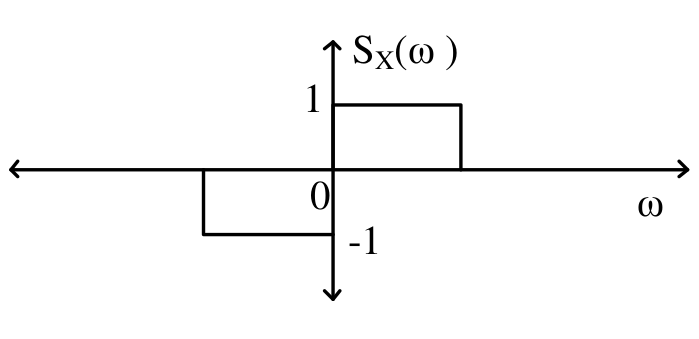
\includegraphics[width=\columnwidth]{ncert/11/16/3/7/figs/fig1.png}
		\caption{CDF of A}
		\label{fig:ncert/11/16/3/7/fig1}
\end{figure}
\begin{figure}[h]
		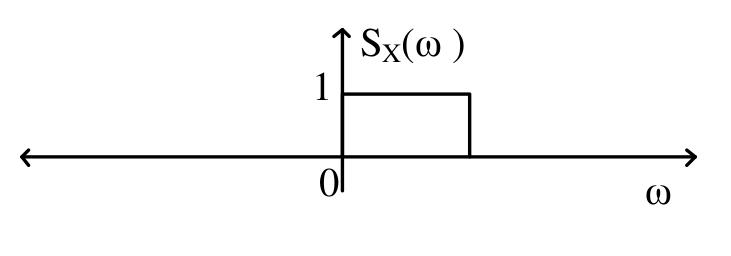
\includegraphics[width=\columnwidth]{ncert/11/16/3/7/figs/fig2.png}
		\caption{PMF of A}
		\label{fig:ncert/11/16/3/7/fig2}
\end{figure}




\item A black and a red dice are rolled.
\begin{enumerate}
    \item Find the conditional probability of obtaining a sum greater than 9, given
that the black die resulted in a 5.
    \item Find the conditional probability of obtaining the sum 8, given that the red die
resulted in a number less than 4.
\end{enumerate}
		\solution
		\iffalse
\let\negmedspace\undefined
\let\negthickspace\undefined
\documentclass[journal,12pt,twocolumn]{IEEEtran}
%\documentclass[conference]{IEEEtran}
%\IEEEoverridecommandlockouts
% The preceding line is only needed to identify funding in the first footnote. If that is unneeded, please comment it out.
\usepackage{cite}
\usepackage{amsmath,amssymb,amsfonts,amsthm}
\usepackage{algorithmic}
\usepackage{graphicx}
\usepackage{textcomp}
\usepackage{xcolor}
\usepackage{txfonts}
\usepackage{listings}
\usepackage{enumitem}
\usepackage{mathtools}
\usepackage{gensymb}
\usepackage[breaklinks=true]{hyperref}
\usepackage{tkz-euclide} % loads  TikZ and tkz-base
\usepackage{listings}
%
%\usepackage{setspace}
%\usepackage{gensymb}
%\doublespacing
%\singlespacing

%\usepackage{graphicx}
%\usepackage{amssymb}
%\usepackage{relsize}
%\usepackage[cmex10]{amsmath}
%\usepackage{amsthm}
%\interdisplaylinepenalty=2500
%\savesymbol{iint}
%\usepackage{txfonts}
%\restoresymbol{TXF}{iint}
%\usepackage{wasysym}
%\usepackage{amsthm}
%\usepackage{iithtlc}
%\usepackage{mathrsfs}
%\usepackage{txfonts}
%\usepackage{stfloats}
%\usepackage{bm}
%\usepackage{cite}
%\usepackage{cases}
%\usepackage{subfig}
%\usepackage{xtab}
%\usepackage{longtable}
%\usepackage{multirow}
%\usepackage{algorithm}
%\usepackage{algpseudocode}
%\usepackage{enumitem}
%\usepackage{mathtools}
%\usepackage{tikz}
%\usepackage{circuitikz}
%\usepackage{verbatim}
%\usepackage{tfrupee}
%\usepackage{stmaryrd}
%\usetkzobj{all}
%    \usepackage{color}                                            %%
%    \usepackage{array}                                            %%
%    \usepackage{longtable}                                        %%
%    \usepackage{calc}                                             %%
%    \usepackage{multirow}                                         %%
%    \usepackage{hhline}                                           %%
%    \usepackage{ifthen}                                           %%
  %optionally (for landscape tables embedded in another document): %%
%    \usepackage{lscape}     
%\usepackage{multicol}
%\usepackage{chngcntr}
%\usepackage{enumerate}

\providecommand{\mbf}{\mathbf}
\providecommand{\pr}[1]{\ensuremath{\Pr\left(#1\right)}}
\providecommand{\qfunc}[1]{\ensuremath{Q\left(#1\right)}}
\providecommand{\sbrak}[1]{\ensuremath{{}\left[#1\right]}}
\providecommand{\lsbrak}[1]{\ensuremath{{}\left[#1\right.}}
\providecommand{\rsbrak}[1]{\ensuremath{{}\left.#1\right]}}
\providecommand{\brak}[1]{\ensuremath{\left(#1\right)}}
\providecommand{\lbrak}[1]{\ensuremath{\left(#1\right.}}
\providecommand{\rbrak}[1]{\ensuremath{\left.#1\right)}}
\providecommand{\cbrak}[1]{\ensuremath{\left\{#1\right\}}}
\providecommand{\lcbrak}[1]{\ensuremath{\left\{#1\right.}}
\providecommand{\rcbrak}[1]{\ensuremath{\left.#1\right\}}}
\theoremstyle{remark}
\newtheorem{rem}{Remark}
\newcommand{\sgn}{\mathop{\mathrm{sgn}}}
%\providecommand{\abs}[1]{\left\vert#1\right\vert}
\providecommand{\res}[1]{\Res\displaylimits_{#1}} 
%\providecommand{\norm}[1]{\left\lVert#1\right\rVert}
%\providecommand{\norm}[1]{\lVert#1\rVert}
\providecommand{\mtx}[1]{\mathbf{#1}}
\providecommand{\mean}[1]{E\left[ #1 \right]}
\providecommand{\fourier}{\overset{\mathcal{F}}{ \rightleftharpoons}}
%\providecommand{\hilbert}{\overset{\mathcal{H}}{ \rightleftharpoons}}
\providecommand{\system}{\overset{\mathcal{H}}{ \longleftrightarrow}}
	%\newcommand{\solution}[2]{\textbf{Solution:}{#1}}
\newcommand{\solution}{\noindent \textbf{Solution: }}
\newcommand{\cosec}{\,\text{cosec}\,}
\providecommand{\dec}[2]{\ensuremath{\overset{#1}{\underset{#2}{\gtrless}}}}
\newcommand{\myvec}[1]{\ensuremath{\begin{pmatrix}#1\end{pmatrix}}}
\newcommand{\mydet}[1]{\ensuremath{\begin{vmatrix}#1\end{vmatrix}}}
%\usepackage{wasysym}
%\newcounter{MYtempeqncnt}
\DeclareMathOperator*{\Res}{Res}
%\renewcommand{\baselinestretch}{2}
\renewcommand\thesection{\arabic{section}}
\renewcommand\thesubsection{\thesection.\arabic{subsection}}
\renewcommand\thesubsubsection{\thesubsection.\arabic{subsubsection}}

\renewcommand\thesectiondis{\arabic{section}}
\renewcommand\thesubsectiondis{\thesectiondis.\arabic{subsection}}
\renewcommand\thesubsubsectiondis{\thesubsectiondis.\arabic{subsubsection}}
%new commands 
\newcommand{\permcomb}[4][0mu]{{{}^{#3}\mkern#1#2_{#4}}}
\newcommand{\comb}[1][-1mu]{\permcomb[#1]{C}}

% correct bad hyphenation here
\hyphenation{op-tical net-works semi-conduc-tor}
\def\inputGnumericTable{}                                 %%

\lstset{
%language=C,
frame=single, 
breaklines=true,
columns=fullflexible
}
%\lstset{
%language=tex,
%frame=single, 
%breaklines=true
%}

\title{

  Assignment:- 2\\
  \Large AI1110: Probability and Random Variables\\
  \Large Indian Institute of Technology, Hyderabad
}
\author{
  CS22BTECH11017\\[4pt]
  Dikshant Khandelwal\\
  12th May, 2023
  % <-this % stops a space
}
\begin{document}
%

\maketitle

\textbf{Exercise 12.13.1.10} 

\textbf{Solution.} 
\fi
Let $X$ and $Y$ be i.i.d, denoting the number which comes up on black and red die respectively.
\begin{align}
    \label{eq:12/13/1/10/cdf}F_{X}(i) = F_{Y}(i) = 
              \begin{cases} 0  & i<1\\
                            \frac{i}{6} & 0 < i \le 6\\
                            1 & i> 6
              \end{cases}
\end{align}
Since
$X$ and $Y$ are independent random variables.
\begin{align}
    \pr{X =k , Y =r} &= \pr{X = k} \pr{Y= r}\\
	\implies p_{X,Y}(k,r) &= \frac{1}{36}
\end{align}
%
\begin{enumerate}
    \item
    \begin{align}
        \pr{X+Y> 9 | X = 5} &= \frac{\pr{X+Y> 9, X = 5}}{\pr{X = 5}}\\
&= \frac{\pr{Y> 4, X = 5}}{\pr{X = 5}}
	    = \frac{\pr{6 \ge Y> 4} \pr{X = 5}}{\pr{X = 5}}\\
			  &= 1 -F_{Y}(4)
                          = \frac{1}{3} 
    \end{align}
\item
From 
  \figref{fig:ncert/12/13/1/10/1},
\begin{align}
	X+Y = 8, Y<4 = (2,6) + (5,3)
\end{align}
Thus, 
\begin{align}
	\pr{X+Y = 8, Y<4} &= p_{X,Y}(2,6)+p_{X,Y}(5,3)
         =\frac{2}{36} 
	 \\
    \implies \pr{X+Y = 8 | Y < 4} &= 
 \frac{\pr{X+Y = 8, Y < 4}}{\pr{Y < 4}}
 \\
	&=
\frac{{\frac{2}{36}}}{\frac{1}{2}}
    =\frac{1}{9} 
    \end{align}
\begin{figure}[h!]
  \centering 
\includegraphics[width= \columnwidth]{ncert/12/13/1/10/figs/figure}
  \caption{$X+Y = 8 | Y < 4$}
  \label{fig:ncert/12/13/1/10/1}
\end{figure}
\end{enumerate}




	\item Given that 2 numbers appearing on throwing two dice are different. Find the probability of the event ‘ the sum of numbers on the dice is 4’ .
		\\
		\solution
		
\let\negmedspace\undefined
\let\negthickspace\undefined
\documentclass[journal,12pt,twocolumn]{IEEEtran}
%\documentclass[conference]{IEEEtran}
%\IEEEoverridecommandlockouts
% The preceding line is only needed to identify funding in the first footnote. If that is unneeded, please comment it out.
\usepackage{cite}
\usepackage{amsmath,amssymb,amsfonts,amsthm}
\usepackage{algorithmic}
\usepackage{graphicx}
\usepackage{textcomp}
\usepackage{xcolor}
\usepackage{txfonts}
\usepackage{listings}
\usepackage{enumitem}
\usepackage{mathtools}
\usepackage{gensymb}
\usepackage[breaklinks=true]{hyperref}
\usepackage{tkz-euclide} % loads  TikZ and tkz-base
\usepackage{listings}
%
%\usepackage{setspace}
%\usepackage{gensymb}
%\doublespacing
%\singlespacing

%\usepackage{graphicx}
%\usepackage{amssymb}
%\usepackage{relsize}
%\usepackage[cmex10]{amsmath}
%\usepackage{amsthm}
%\interdisplaylinepenalty=2500
%\savesymbol{iint}
%\usepackage{txfonts}
%\restoresymbol{TXF}{iint}
%\usepackage{wasysym}
%\usepackage{amsthm}
%\usepackage{iithtlc}
%\usepackage{mathrsfs}
%\usepackage{txfonts}
%\usepackage{stfloats}
%\usepackage{bm}
%\usepackage{cite}
%\usepackage{cases}
%\usepackage{subfig}
%\usepackage{xtab}
%\usepackage{longtable}
%\usepackage{multirow}
%\usepackage{algorithm}
%\usepackage{algpseudocode}
%\usepackage{enumitem}
%\usepackage{mathtools}
%\usepackage{tikz}
%\usepackage{circuitikz}
%\usepackage{verbatim}
%\usepackage{tfrupee}
%\usepackage{stmaryrd}
%\usetkzobj{all}
%    \usepackage{color}                                            %%
%    \usepackage{array}                                            %%
%    \usepackage{longtable}                                        %%
%    \usepackage{calc}                                             %%
%    \usepackage{multirow}                                         %%
%    \usepackage{hhline}                                           %%
%    \usepackage{ifthen}                                           %%
  %optionally (for landscape tables embedded in another document): %%
%    \usepackage{lscape}     
%\usepackage{multicol}
%\usepackage{chngcntr}
%\usepackage{enumerate}

\providecommand{\mbf}{\mathbf}
\providecommand{\pr}[1]{\ensuremath{\Pr\left(#1\right)}}
\providecommand{\qfunc}[1]{\ensuremath{Q\left(#1\right)}}
\providecommand{\sbrak}[1]{\ensuremath{{}\left[#1\right]}}
\providecommand{\lsbrak}[1]{\ensuremath{{}\left[#1\right.}}
\providecommand{\rsbrak}[1]{\ensuremath{{}\left.#1\right]}}
\providecommand{\brak}[1]{\ensuremath{\left(#1\right)}}
\providecommand{\lbrak}[1]{\ensuremath{\left(#1\right.}}
\providecommand{\rbrak}[1]{\ensuremath{\left.#1\right)}}
\providecommand{\cbrak}[1]{\ensuremath{\left\{#1\right\}}}
\providecommand{\lcbrak}[1]{\ensuremath{\left\{#1\right.}}
\providecommand{\rcbrak}[1]{\ensuremath{\left.#1\right\}}}
\theoremstyle{remark}
\newtheorem{rem}{Remark}
\newcommand{\sgn}{\mathop{\mathrm{sgn}}}
%\providecommand{\abs}[1]{\left\vert#1\right\vert}
\providecommand{\res}[1]{\Res\displaylimits_{#1}} 
%\providecommand{\norm}[1]{\left\lVert#1\right\rVert}
%\providecommand{\norm}[1]{\lVert#1\rVert}
\providecommand{\mtx}[1]{\mathbf{#1}}
\providecommand{\mean}[1]{E\left[ #1 \right]}
\providecommand{\fourier}{\overset{\mathcal{F}}{ \rightleftharpoons}}
%\providecommand{\hilbert}{\overset{\mathcal{H}}{ \rightleftharpoons}}
\providecommand{\system}{\overset{\mathcal{H}}{ \longleftrightarrow}}
	%\newcommand{\solution}[2]{\textbf{Solution:}{#1}}
\newcommand{\solution}{\noindent \textbf{Solution: }}
\newcommand{\cosec}{\,\text{cosec}\,}
\providecommand{\dec}[2]{\ensuremath{\overset{#1}{\underset{#2}{\gtrless}}}}
\newcommand{\myvec}[1]{\ensuremath{\begin{pmatrix}#1\end{pmatrix}}}
\newcommand{\mydet}[1]{\ensuremath{\begin{vmatrix}#1\end{vmatrix}}}
%\usepackage{wasysym}
%\newcounter{MYtempeqncnt}
\DeclareMathOperator*{\Res}{Res}
%\renewcommand{\baselinestretch}{2}
\renewcommand\thesection{\arabic{section}}
\renewcommand\thesubsection{\thesection.\arabic{subsection}}
\renewcommand\thesubsubsection{\thesubsection.\arabic{subsubsection}}

\renewcommand\thesectiondis{\arabic{section}}
\renewcommand\thesubsectiondis{\thesectiondis.\arabic{subsection}}
\renewcommand\thesubsubsectiondis{\thesubsectiondis.\arabic{subsubsection}}
%new commands 
\newcommand{\permcomb}[4][0mu]{{{}^{#3}\mkern#1#2_{#4}}}
\newcommand{\comb}[1][-1mu]{\permcomb[#1]{C}}
\providecommand{\cond}[2]{#1\middle|#2}

% correct bad hyphenation here
\hyphenation{op-tical net-works semi-conduc-tor}
\def\inputGnumericTable{}                                 %%

\lstset{
%language=C,
frame=single, 
breaklines=true,
columns=fullflexible
}
%\lstset{
%language=tex,
%frame=single, 
%breaklines=true
%}

\title{

  Assignment:- 3\\
  \Large AI1110: Probability and Random Variables\\
  \Large Indian Institute of Technology, Hyderabad
}
\author{
  CS22BTECH11017\\[4pt]
  Dikshant Khandelwal\\
  17th May, 2023
  % <-this % stops a space
}
\begin{document}
%

\maketitle

\textbf{Exercise 12.13.1.14}
Given that 2 numbers appearing on throwing two dice are different. Find the probability of the event ‘ the sum of numbers on the dice is 4’ .

\textbf{Solution.} Let $X$ and $Y$ be two random variables.

\begin{table}[h]
    \label{tab:0}
    %%%%%%%%%%%%%%%%%%%%%%%%%%%%%%%%%%%%%%%%%%%%%%%%%%%%%%%%%%%%%%%%%%%%%%
%%                                                                  %%
%%  This is the header of a LaTeX2e file exported from Gnumeric.    %%
%%                                                                  %%
%%  This file can be compiled as it stands or included in another   %%
%%  LaTeX document. The table is based on the longtable package so  %%
%%  the longtable options (headers, footers...) can be set in the   %%
%%  preamble section below (see PRAMBLE).                           %%
%%                                                                  %%
%%  To include the file in another, the following two lines must be %%
%%  in the including file:                                          %%
%%        \def\inputGnumericTable{}                                 %%
%%  at the beginning of the file and:                               %%
%%        \input{name-of-this-file.tex}                             %%
%%  where the table is to be placed. Note also that the including   %%
%%  file must use the following packages for the table to be        %%
%%  rendered correctly:                                             %%
%%    \usepackage[latin1]{inputenc}                                 %%
%%    \usepackage{color}                                            %%
%%    \usepackage{array}                                            %%
%%    \usepackage{longtable}                                        %%
%%    \usepackage{calc}                                             %%
%%    \usepackage{multirow}                                         %%
%%    \usepackage{hhline}                                           %%
%%    \usepackage{ifthen}                                           %%
%%  optionally (for landscape tables embedded in another document): %%
%%    \usepackage{lscape}                                           %%
%%                                                                  %%
%%%%%%%%%%%%%%%%%%%%%%%%%%%%%%%%%%%%%%%%%%%%%%%%%%%%%%%%%%%%%%%%%%%%%%



%%  This section checks if we are begin input into another file or  %%
%%  the file will be compiled alone. First use a macro taken from   %%
%%  the TeXbook ex 7.7 (suggestion of Han-Wen Nienhuys).            %%
\def\ifundefined#1{\expandafter\ifx\csname#1\endcsname\relax}


%%  Check for the \def token for inputed files. If it is not        %%
%%  defined, the file will be processed as a standalone and the     %%
%%  preamble will be used.                                          %%
\ifundefined{inputGnumericTable}

%%  We must be able to close or not the document at the end.        %%
	\def\gnumericTableEnd{\end{document}}


%%%%%%%%%%%%%%%%%%%%%%%%%%%%%%%%%%%%%%%%%%%%%%%%%%%%%%%%%%%%%%%%%%%%%%
%%                                                                  %%
%%  This is the PREAMBLE. Change these values to get the right      %%
%%  paper size and other niceties.                                  %%
%%                                                                  %%
%%%%%%%%%%%%%%%%%%%%%%%%%%%%%%%%%%%%%%%%%%%%%%%%%%%%%%%%%%%%%%%%%%%%%%

	\documentclass[12pt%
			  %,landscape%
                    ]{report}
       \usepackage[latin1]{inputenc}
       \usepackage{fullpage}
       \usepackage{color}
       \usepackage{array}
       \usepackage{longtable}
       \usepackage{calc}
       \usepackage{multirow}
       \usepackage{hhline}
       \usepackage{ifthen}

	\begin{document}


%%  End of the preamble for the standalone. The next section is for %%
%%  documents which are included into other LaTeX2e files.          %%
\else

%%  We are not a stand alone document. For a regular table, we will %%
%%  have no preamble and only define the closing to mean nothing.   %%
    \def\gnumericTableEnd{}

%%  If we want landscape mode in an embedded document, comment out  %%
%%  the line above and uncomment the two below. The table will      %%
%%  begin on a new page and run in landscape mode.                  %%
%       \def\gnumericTableEnd{\end{landscape}}
%       \begin{landscape}


%%  End of the else clause for this file being \input.              %%
\fi

%%%%%%%%%%%%%%%%%%%%%%%%%%%%%%%%%%%%%%%%%%%%%%%%%%%%%%%%%%%%%%%%%%%%%%
%%                                                                  %%
%%  The rest is the gnumeric table, except for the closing          %%
%%  statement. Changes below will alter the table's appearance.     %%
%%                                                                  %%
%%%%%%%%%%%%%%%%%%%%%%%%%%%%%%%%%%%%%%%%%%%%%%%%%%%%%%%%%%%%%%%%%%%%%%

\providecommand{\gnumericmathit}[1]{#1} 
%%  Uncomment the next line if you would like your numbers to be in %%
%%  italics if they are italizised in the gnumeric table.           %%
%\renewcommand{\gnumericmathit}[1]{\mathit{#1}}
\providecommand{\gnumericPB}[1]%
{\let\gnumericTemp=\\#1\let\\=\gnumericTemp\hspace{0pt}}
 \ifundefined{gnumericTableWidthDefined}
        \newlength{\gnumericTableWidth}
        \newlength{\gnumericTableWidthComplete}
        \newlength{\gnumericMultiRowLength}
        \global\def\gnumericTableWidthDefined{}
 \fi
%% The following setting protects this code from babel shorthands.  %%
 \ifthenelse{\isundefined{\languageshorthands}}{}{\languageshorthands{english}}
%%  The default table format retains the relative column widths of  %%
%%  gnumeric. They can easily be changed to c, r or l. In that case %%
%%  you may want to comment out the next line and uncomment the one %%
%%  thereafter                                                      %%
\providecommand\gnumbox{\makebox[0pt]}
%%\providecommand\gnumbox[1][]{\makebox}

%% to adjust positions in multirow situations                       %%
\setlength{\bigstrutjot}{\jot}
\setlength{\extrarowheight}{\doublerulesep}

%%  The \setlongtables command keeps column widths the same across  %%
%%  pages. Simply comment out next line for varying column widths.  %%
\setlongtables

\setlength\gnumericTableWidth{%
	85pt+%
	53pt+%
	178pt+%
0pt}
\def\gumericNumCols{3}
\setlength\gnumericTableWidthComplete{\gnumericTableWidth+%
         \tabcolsep*\gumericNumCols*2+\arrayrulewidth*\gumericNumCols}
\ifthenelse{\lengthtest{\gnumericTableWidthComplete > \linewidth}}%
         {\def\gnumericScale{1*\ratio{\linewidth-%
                        \tabcolsep*\gumericNumCols*2-%
                        \arrayrulewidth*\gumericNumCols}%
{\gnumericTableWidth}}}%
{\def\gnumericScale{1}}

%%%%%%%%%%%%%%%%%%%%%%%%%%%%%%%%%%%%%%%%%%%%%%%%%%%%%%%%%%%%%%%%%%%%%%
%%                                                                  %%
%% The following are the widths of the various columns. We are      %%
%% defining them here because then they are easier to change.       %%
%% Depending on the cell formats we may use them more than once.    %%
%%                                                                  %%
%%%%%%%%%%%%%%%%%%%%%%%%%%%%%%%%%%%%%%%%%%%%%%%%%%%%%%%%%%%%%%%%%%%%%%

\ifthenelse{\isundefined{\gnumericColA}}{\newlength{\gnumericColA}}{}\settowidth{\gnumericColA}{\begin{tabular}{@{}p{85pt*\gnumericScale}@{}}x\end{tabular}}
\ifthenelse{\isundefined{\gnumericColB}}{\newlength{\gnumericColB}}{}\settowidth{\gnumericColB}{\begin{tabular}{@{}p{53pt*\gnumericScale}@{}}x\end{tabular}}
\ifthenelse{\isundefined{\gnumericColC}}{\newlength{\gnumericColC}}{}\settowidth{\gnumericColC}{\begin{tabular}{@{}p{178pt*\gnumericScale}@{}}x\end{tabular}}

\begin{tabular}[c]{%
	b{\gnumericColA}%
	b{\gnumericColB}%
	b{\gnumericColC}%
	}

%%%%%%%%%%%%%%%%%%%%%%%%%%%%%%%%%%%%%%%%%%%%%%%%%%%%%%%%%%%%%%%%%%%%%%
%%  The longtable options. (Caption, headers... see Goosens, p.124) %%
%	\caption{The Table Caption.}             \\	%
% \hline	% Across the top of the table.
%%  The rest of these options are table rows which are placed on    %%
%%  the first, last or every page. Use \multicolumn if you want.    %%

%%  Header for the first page.                                      %%
%	\multicolumn{3}{c}{The First Header} \\ \hline 
%	\multicolumn{1}{c}{colTag}	%Column 1
%	&\multicolumn{1}{c}{colTag}	%Column 2
%	&\multicolumn{1}{c}{colTag}	\\ \hline %Last column
%	\endfirsthead

%%  The running header definition.                                  %%
%	\hline
%	\multicolumn{3}{l}{\ldots\small\slshape continued} \\ \hline
%	\multicolumn{1}{c}{colTag}	%Column 1
%	&\multicolumn{1}{c}{colTag}	%Column 2
%	&\multicolumn{1}{c}{colTag}	\\ \hline %Last column
%	\endhead

%%  The running footer definition.                                  %%
%	\hline
%	\multicolumn{3}{r}{\small\slshape continued\ldots} \\
%	\endfoot

%%  The ending footer definition.                                   %%
%	\multicolumn{3}{c}{That's all folks} \\ \hline 
%	\endlastfoot
%%%%%%%%%%%%%%%%%%%%%%%%%%%%%%%%%%%%%%%%%%%%%%%%%%%%%%%%%%%%%%%%%%%%%%

\hhline{|-|-|-}
	 \multicolumn{1}{|p{\gnumericColA}|}%
	{\gnumericPB{\centering}\gnumbox{\textbf{Parameter}}}
	&\multicolumn{1}{p{\gnumericColB}|}%
	{\gnumericPB{\centering}\gnumbox{\textbf{Value}}}
	&\multicolumn{1}{p{\gnumericColC}|}%
	{\gnumericPB{\centering}\gnumbox{\textbf{Description}}}
\\
\hhline{|---|}
	 \multicolumn{1}{|p{\gnumericColA}|}%
	{\gnumericPB{\centering}\gnumbox{$n$}}
	&\multicolumn{1}{p{\gnumericColB}|}%
	{\gnumericPB{\centering}\gnumbox{$n$}}
	&\multicolumn{1}{p{\gnumericColC}|}%
	{\gnumericPB{\centering}\gnumbox{number of coin tosses}}
\\
\hhline{|---|}
	 \multicolumn{1}{|p{\gnumericColA}|}%
	{\gnumericPB{\centering}\gnumbox{$p$}}
	&\multicolumn{1}{p{\gnumericColB}|}%
	{\gnumericPB{\centering}\gnumbox{$\frac{1}{2}$}}
	&\multicolumn{1}{p{\gnumericColC}|}%
	{\gnumericPB{\centering}\gnumbox{getting a head on a coin toss}}
\\
\hhline{|---|}
	 \multicolumn{1}{|p{\gnumericColA}|}%
	{\gnumericPB{\centering}\gnumbox{$q$}}
	&\multicolumn{1}{p{\gnumericColB}|}%
	{\gnumericPB{\centering}\gnumbox{$\frac{1}{2}$}}
	&\multicolumn{1}{p{\gnumericColC}|}%
	{\gnumericPB{\centering}\gnumbox{getting a tail on a coin toss}}
\\
\hhline{|---|}
	 \multicolumn{1}{|p{\gnumericColA}|}%
	{\gnumericPB{\centering}\gnumbox{$\mu = np$}}
	&\multicolumn{1}{p{\gnumericColB}|}%
	{\gnumericPB{\centering}\gnumbox{$\frac{n}{2}$}}
	&\multicolumn{1}{p{\gnumericColC}|}%
	{\gnumericPB{\centering}\gnumbox{mean of the distribution}}
\\
\hhline{|---|}
	 \multicolumn{1}{|p{\gnumericColA}|}%
	{\gnumericPB{\centering}\gnumbox{${\sigma}^2 = npq$}}
	&\multicolumn{1}{p{\gnumericColB}|}%
	{\gnumericPB{\centering}\gnumbox{$\frac{n}{4}$}}
	&\multicolumn{1}{p{\gnumericColC}|}%
	{\gnumericPB{\centering}\gnumbox{variance of the distribution}}
\\
\hhline{|---|}
	 \multicolumn{1}{|p{\gnumericColA}|}%
	{\gnumericPB{\centering}\gnumbox{$Y$}}
	&\multicolumn{1}{p{\gnumericColB}|}%
	{\gnumericPB{\centering}\gnumbox{$\geq 1$}}
	&\multicolumn{1}{p{\gnumericColC}|}%
	{\gnumericPB{\centering}\gnumbox{Number of heads}}
\\
\hhline{|-|-|-|}

\end{tabular}

\ifthenelse{\isundefined{\languageshorthands}}{}{\languageshorthands{\languagename}}
\gnumericTableEnd

    \caption{Random Variables for Die Rolls}
   \end{table}

\begin{align}
    \pr{\cond{X+Y = 4}{X \neq Y}} &= \frac{\pr{X+Y = 4,X \neq Y}}{\pr{X\neq Y}}
\end{align}

Probability of an event $E$, written as $\pr{E}$
\begin{align}
\pr{E}=\frac{\text{Number of outcomes favourable to $E$}}{\text{Total Number of possible outcomes }}
\end{align}

\begin{align}
    \pr{X\neq Y} &= 1 - \pr{X = Y}\\
    &= 1 - \frac{6}{36}\\
    &= \frac{5}{6}
\end{align}

Let $A$ and $B$ be two events.
\begin{table}[h]
  \label{tab:1}
  \begin{tabular}{|l|l|l|}\hline
     &$X_1$ &$X_2$ \\\hline
E:   &1 &1	\\\hline
F:   &1 &1	\\\hline
\end{tabular}

  \caption{Events A and B}
 \end{table}
\begin{align}
    A &= A(B + B^{\prime})\\
       &= AB + AB^{\prime}\\
       \therefore \pr{A} &= \pr{AB} + \pr{AB^{\prime}}\\
       \pr{AB}  &= \pr{A}-\pr{AB^{\prime}}
\end{align}



 
\begin{align}
 X &= Y\\
 X+Y &= 4\\
 X &= Y =2\\
  \therefore  \pr{AB^{\prime}} &= \pr{X+Y = 4,X = Y} = \frac{1}{36}
\end{align}



\begin{align}
\pr{X+Y = n} &= 
\begin{cases}
0 & n < 1
\\
\frac{n-1}{36} &  2 \le n \le  7
\\
\frac{13-n}{36} & 7 < n \le 12
\\
0 & n > 12
\end{cases}
\end{align}

\begin{align}
    \therefore \pr{A} = \pr{X+Y = 4} = \frac{4-1}{36} = \frac{1}{12}
\end{align}


\begin{align}
    \pr{AB} = \pr{X + Y = 4 , X \ne Y} &= \frac{1}{12} - \frac{1}{36}\\
                        &= \frac{1}{18}
\end{align}

\begin{align}
  \pr{\cond{X+Y = 4}{X \neq Y}} &= \frac{\brak{\frac{1}{18}}}{\brak{\frac{5}{6}}}\\
    \therefore \pr{\cond{X+Y = 4}{X \neq Y}} &= \frac{1}{15}
\end{align}
\end{document}



 \item If each element of a $2\times 2$ determinant is either zero or one. What is the probability that the value of the determinant is positive ? 
 (Assume that the individual entries of the determinant are chosen independently each value being assumed with probability $\frac{1}{2}$) \\
 \solution
		\iffalse
\let\negmedspace\undefined 
 \let\negthickspace\undefined 
 \documentclass[journal,12pt,onecolumn]{IEEEtran} 
 %\documentclass[conference]{IEEEtran} 
 %\IEEEoverridecommandlockouts 
 % The preceding line is only needed to identify funding in the first footnote. If that is unneeded, please comment it out. 
 \usepackage{cite} 
 \usepackage{amsmath,amssymb,amsfonts,amsthm} 
 \usepackage{algorithmic} 
 \usepackage{graphicx} 
 \usepackage{textcomp} 
 \usepackage{xcolor} 
 \usepackage{txfonts} 
 \usepackage{listings} 
 \usepackage{enumitem} 
 \usepackage{mathtools} 
 \usepackage{gensymb} 
 \usepackage[breaklinks=true]{hyperref} 
 \usepackage{tkz-euclide} % loads  TikZ and tkz-base 
 \usepackage{listings} 
 \usepackage{caption}
 % 
 %\usepackage{setspace} 
 %\usepackage{gensymb} 
 %\doublespacing 
 %\singlespacing 
  
 %\usepackage{graphicx} 
 %\usepackage{amssymb} 
 %\usepackage{relsize} 
  %\usepackage[cmex10]{amsmath} 
 %\usepackage{amsthm} 
 %\interdisplaylinepenalty=2500 
 %\savesymbol{iint} 
 %\usepackage{txfonts} 
 %\restoresymbol{TXF}{iint} 
 %\usepackage{wasysym} 
 %\usepackage{amsthm} 
 %\usepackage{iithtlc} 
 %\usepackage{mathrsfs} 
 %\usepackage{txfonts} 
 %\usepackage{stfloats} 
 %\usepackage{bm} 
 %\usepackage{cite} 
 %\usepackage{cases} 
 %\usepackage{subfig} 
 %\usepackage{xtab} 
 %\usepackage{longtable} 
 %\usepackage{multirow} 
 %\usepackage{algorithm} 
 %\usepackage{algpseudocode} 
 %\usepackage{enumitem} 
 %\usepackage{mathtools} 
 %\usepackage{tikz} 
 %\usepackage{circuitikz} 
 %\usepackage{verbatim} 
 %\usepackage{tfrupee} 
 %\usepackage{stmaryrd} 
 %\usetkzobj{all} 
 %    \usepackage{color}                                            %% 
 %    \usepackage{array}                                            %% 
 %    \usepackage{longtable}                                        %% 
 %    \usepackage{calc}                                             %% 
 %    \usepackage{multirow}                                         %% 
 %    \usepackage{hhline}                                           %% 
 %    \usepackage{ifthen}                                           %% 
   %optionally (for landscape tables embedded in another document): %% 
 %    \usepackage{lscape}      
 %\usepackage{multicol} 
 %\usepackage{chngcntr} 
 %\usepackage{enumerate} 
  
 %\usepackage{wasysym} 
 %\newcounter{MYtempeqncnt} 
 \DeclareMathOperator*{\Res}{Res} 
 %\renewcommand{\baselinestretch}{2} 
 \renewcommand\thesection{\arabic{section}} 
 \renewcommand\thesubsection{\thesection.\arabic{subsection}} 
 \renewcommand\thesubsubsection{\thesubsection.\arabic{subsubsection}} 
  
 \renewcommand\thesectiondis{\arabic{section}} 
 \renewcommand\thesubsectiondis{\thesectiondis.\arabic{subsection}} 
 \renewcommand\thesubsubsectiondis{\thesubsectiondis.\arabic{subsubsection}} 
  
 % correct bad hyphenation here 
 \hyphenation{op-tical net-works semi-conduc-tor} 
 \def\inputGnumericTable{}                                 %% 
  
 \lstset{ 
 %language=C, 
 frame=single,  
 breaklines=true, 
 columns=fullflexible 
 } 
 %\lstset{ 
 %language=tex, 
 %frame=single,  
 %breaklines=true 
 %} 
  
 \begin{document} 
 % 
  
  
 \newtheorem{theorem}{Theorem}[section] 
 \newtheorem{problem}{Problem} 
 \newtheorem{proposition}{Proposition}[section] 
 \newtheorem{lemma}{Lemma}[section] 
 \newtheorem{corollary}[theorem]{Corollary} 
 \newtheorem{example}{Example}[section] 
 \newtheorem{definition}[problem]{Definition} 
 %\newtheorem{thm}{Theorem}[section]  
 %\newtheorem{defn}[thm]{Definition} 
 %\newtheorem{algorithm}{Algorithm}[section] 
 %\newtheorem{cor}{Corollary} 
 \newcommand{\BEQA}{\begin{eqnarray}} 
 \newcommand{\EEQA}{\end{eqnarray}} 
 \newcommand{\define}{\stackrel{\triangle}{=}} 
  
 \bibliographystyle{IEEEtran} 
 %\bibliographystyle{ieeetr} 
  
  
 \providecommand{\mbf}{\mathbf} 
 \providecommand{\pr}[1]{\ensuremath{\Pr\left(#1\right)}} 
 \providecommand{\qfunc}[1]{\ensuremath{Q\left(#1\right)}} 
 \providecommand{\sbrak}[1]{\ensuremath{{}\left[#1\right]}} 
 \providecommand{\lsbrak}[1]{\ensuremath{{}\left[#1\right.}} 
 \providecommand{\rsbrak}[1]{\ensuremath{{}\left.#1\right]}} 
 \providecommand{\brak}[1]{\ensuremath{\left(#1\right)}} 
 \providecommand{\lbrak}[1]{\ensuremath{\left(#1\right.}} 
 \providecommand{\rbrak}[1]{\ensuremath{\left.#1\right)}} 
 \providecommand{\cbrak}[1]{\ensuremath{\left\{#1\right\}}} 
 \providecommand{\lcbrak}[1]{\ensuremath{\left\{#1\right.}} 
 \providecommand{\rcbrak}[1]{\ensuremath{\left.#1\right\}}} 
 \theoremstyle{remark} 
 \newtheorem{rem}{Remark} 
 \newcommand{\sgn}{\mathop{\mathrm{sgn}}} 
 \providecommand{\abs}[1]{\left\vert#1\right\vert} 
 \providecommand{\res}[1]{\Res\displaylimits_{#1}}  
 \providecommand{\norm}[1]{\left\lVert#1\right\rVert} 
 %\providecommand{\norm}[1]{\lVert#1\rVert} 
 \providecommand{\mtx}[1]{\mathbf{#1}} 
 \providecommand{\mean}[1]{E\left[ #1 \right]} 
 \providecommand{\fourier}{\overset{\mathcal{F}}{ \rightleftharpoons}} 
 %\providecommand{\hilbert}{\overset{\mathcal{H}}{ \rightleftharpoons}} 
 \providecommand{\system}{\overset{\mathcal{H}}{ \longleftrightarrow}} 
         %\newcommand{\solution}[2]{\textbf{Solution:}{#1}} 
 \newcommand{\solution}{\noindent \textbf{Solution: }} 
 \newcommand{\cosec}{\,\text{cosec}\,} 
 \providecommand{\dec}[2]{\ensuremath{\overset{#1}{\underset{#2}{\gtrless}}}} 
 \newcommand{\myvec}[1]{\ensuremath{\begin{pmatrix}#1\end{pmatrix}}} 
 \newcommand{\mydet}[1]{\ensuremath{\begin{vmatrix}#1\end{vmatrix}}} 
 %\numberwithin{equation}{section} 
 %\numberwithin{equation}{subsection} 
 %\numberwithin{problem}{section} 
 %\numberwithin{definition}{section} 
 %\makeatletter 
 %\@addtoreset{figure}{problem} 
 %\makeatother 
  
 %\let\StandardTheFigure\thefigure 
 \let\vec\mathbf 
 %\renewcommand{\thefigure}{\theproblem.\arabic{figure}} 
 %\renewcommand{\thefigure}{\theproblem} 
 %\setlist[enumerate,1]{before=\renewcommand\theequation{\theenumi.\arabic{equation}} 
 %\counterwithin{equation}{enumi} 
  
  
 %\renewcommand{\theequation}{\arabic{subsection}.\arabic{equation}} 
  
 %\def\putbox#1#2#3{\makebox[0in][l]{\makebox[#1][l]{}\raisebox{\baselineskip}[0in][0in]{\raisebox{#2}[0in][0in]{#3}}}} 
 %     \def\rightbox#1{\makebox[0in][r]{#1}} 
 %     \def\centbox#1{\makebox[0in]{#1}} 
 %     \def\topbox#1{\raisebox{-\baselineskip}[0in][0in]{#1}} 
 %     \def\midbox#1{\raisebox{-0.5\baselineskip}[0in][0in]{#1}} 
   
 \vspace{3cm} 
  
 \title{ Assignment 2 
  
         \Large AI1110: Probability and Random Variables 
  
          INDIAN INSTITUTE OF TECHNOLOGY, HYDERABAD 
 } 
 \author{ LAHARI GUNTI 
          
         AI22BTECH11008 
 } 
  
 \maketitle 
  
 \bigskip 
 \renewcommand{\thefigure}{\theenumi} 
 \renewcommand{\thetable}{\theenumi} 
 \textbf{12.13.6.14}: 
 \textbf{Solution}: 
         Let us assume the $2*2$ determinant as 
 \fi
		 Let the matrix be 
		 \begin{align}
			 \myvec{ a & b \\ c & d }
		 \end{align}
 \begin{enumerate} 
	 \item   The desired probability can be expressed as
                         \begin{align} 
				 \pr{ad-bc > 0} &=
				 \pr{a > \frac{bc}{d} }
= 1 - \pr{a \le \frac{bc}{d}} 
\\
				 &= 1- F_A\brak{\frac{bc}{d}} 
                         \end{align} 
		 \item Since
                         \begin{align}
				 F_A\brak{x} &= \begin{cases} 0 &  x = 0, \\ \frac{1}{2} &  0 \leqslant\: x < 1 , \\ 1 &  1 \leqslant\: x < \infty \end{cases},
					\\
				E_d\brak{F_A\brak{\frac{bc}{d}}} &= \frac{1}{2}F_A\brak{bc} + \frac{1}{2}F_A\brak{\infty} 
				= \frac{1}{2}F_A\brak{bc} + \frac{1}{2} 
			 \end{align}
		 \item			 and 
			 \begin{align}
E_b\brak{\frac{1}{2}F_A\brak{bc} + \frac{1}{2}} &= \frac{1}{2}E_b\brak{F_A\brak{bc}} + \frac{1}{2} 
				 = \frac{1}{2}\brak{\frac{1}{2}F_A\brak{0} + \frac{1}{2}F_A\brak{c}} \\
				 &= \frac{1}{2} + \frac{1}{8} + \frac{1}{4}F_A\brak{c} 
				 = \frac{5}{8} + \frac{1}{4}F_A\brak{c}
			 \end{align}
		 \item
			 yielding
			 \begin{align}
				 E_c\brak{\frac{5}{8} + \frac{1}{4}F_A\brak{c}} &= \frac{5}{8} + \frac{1}{4}E_c\brak{F_A\brak{c}} \\
				 &= \frac{5}{8} + \frac{1}{4}\brak{\frac{1}{2}F_A\brak{0} + \frac{1}{2}F_A\brak{1}} \\
				 &= \frac{5}{8} + \frac{1}{4}\brak{\frac{1}{4} + \frac{1}{2}} 
				 = \frac{13}{16}
			 \end{align}
		 \item Thus, the required probability is
			 \begin{align}
				\pr{a > \frac{bc}{d}} = 1 - E_b,c,d\brak{F_A\brak{\frac{bc}{d}}} 
                                                     = 1 - \frac{13}{16} 
						     = \frac{3}{16}
			 \end{align}
 \end{enumerate} 

\item Two customers Shyam and Ekta are visiting a particular shop in the same week(Tuesday to Saturday). Each is equally likely to visit the shop on any day as on another day. What is the probability that both will visit the shop on (i) the same day? (ii) consecutive days? (iii) different days?
\\
	\iffalse
\let\negmedspace\undefined
\let\negthickspace\undefined
\documentclass[journal,12pt,onecolumn]{IEEEtran}
       \def\inputGnumericTable{}                                 %%
\usepackage{cite}
\usepackage{amsmath,amssymb,amsfonts,amsthm}
\usepackage{algorithmic}
\usepackage{graphicx}
\usepackage{textcomp}
\usepackage{xcolor}
\usepackage{txfonts}
\usepackage{listings}
\usepackage{enumitem}
\usepackage{mathtools}
\usepackage{gensymb}
\usepackage[breaklinks=true]{hyperref}
\usepackage{tkz-euclide} % loads  TikZ and tkz-base
\usepackage{listings}
\usepackage{gvv}
%
%\usepackage{setspace}
%\usepackage{gensymb}
%\doublespacing
%\singlespacing

%\usepackage{graphicx}
%\usepackage{amssymb}
%\usepackage{relsize}
%\usepackage[cmex10]{amsmath}
%\usepackage{amsthm}
%\interdisplaylinepenalty=2500
%\savesymbol{iint}
%\usepackage{txfonts}
%\restoresymbol{TXF}{iint}
%\usepackage{wasysym}
%\usepackage{amsthm}
%\usepackage{iithtlc}
%\usepackage{mathrsfs}
%\usepackage{txfonts}
%\usepackage{stfloats}
%\usepackage{bm}
%\usepackage{cite}
%\usepackage{cases}
%\usepackage{subfig}
%\usepackage{xtab}
%\usepackage{longtable}
%\usepackage{multirow}
%\usepackage{algorithm}
%\usepackage{algpseudocode}
%\usepackage{enumitem}
%\usepackage{mathtools}
%\usepackage{tikz}
%\usepackage{circuitikz}
%\usepackage{verbatim}
%\usepackage{tfrupee}
%\usepackage{stmaryrd}
%\usetkzobj{all}
    \usepackage{color}                                            %%
    \usepackage{array}                                            %%
    \usepackage{longtable}                                        %%
    \usepackage{calc}                                             %%
    \usepackage{multirow}                                         %%
    \usepackage{hhline}                                           %%
    \usepackage{ifthen}                                           %%
 %optionally (for landscape tables embedded in another document): %%
    \usepackage{lscape}     
%\usepackage{multicol}
%\usepackage{chngcntr}
%\usepackage{enumerate}

%\usepackage{wasysym}
%\documentclass[conference]{IEEEtran}
%\IEEEoverridecommandlockouts
% The preceding line is only needed to identify funding in the first footnote. If that is unneeded, please comment it out.

\newtheorem{theorem}{Theorem}[section]
\newtheorem{problem}{Problem}
\newtheorem{proposition}{Proposition}[section]
\newtheorem{lemma}{Lemma}[section]
\newtheorem{corollary}[theorem]{Corollary}
\newtheorem{example}{Example}[section]
\newtheorem{definition}[problem]{Definition}
%\newtheorem{thm}{Theorem}[section] 
%\newtheorem{defn}[thm]{Definition}
%\newtheorem{algorithm}{Algorithm}[section]
%\newtheorem{cor}{Corollary}
\newcommand{\BEQA}{\begin{eqnarray}}
\newcommand{\EEQA}{\end{eqnarray}}
\newcommand{\define}{\stackrel{\triangle}{=}}
\theoremstyle{remark}
\newtheorem{rem}{Remark}

%\bibliographystyle{ieeetr}
\begin{document}
%

\bibliographystyle{IEEEtran}


\vspace{3cm}

\title{Solution to 10.15.2.1}
\author{Devansh Jain - EE22BTECH11018}
%\title{
%	\logo{Matrix Analysis through Octave}{\begin{center}\includegraphics[scale=.24]{tlc}\end{center}}{}{HAMDSP}
%}


% paper title
% can use linebreaks \\ within to get better formatting as desired
%\title{Matrix Analysis through Octave}
%
%
% author names and IEEE memberships
% note positions of commas and nonbreaking spaces ( ~ ) LaTeX will not break
% a structure at a ~ so this keeps an author's name from being broken across
% two lines.
% use \thanks{} to gain access to the first footnote area
% a separate \thanks must be used for each paragraph as LaTeX2e's \thanks
% was not built to handle multiple paragraphs
%

%\author{<-this % stops a space
%\thanks{}}
%}
% note the % following the last \IEEEmembership and also \thanks - 
% these prevent an unwanted space from occurring between the last author name
% and the end of the author line. i.e., if you had this:
% 
% \author{....lastname \thanks{...} \thanks{...} }
%                     ^------------^------------^----Do not want these spaces!
%
% a space would be appended to the last name and could cause every name on that
% line to be shifted left slightly. This is one of those "LaTeX things". For
% instance, "\textbf{A} \textbf{B}" will typeset as "A B" not "AB". To get
% "AB" then you have to do: "\textbf{A}\textbf{B}"
% \thanks is no different in this regard, so shield the last } of each \thanks
% that ends a line with a % and do not let a space in before the next \thanks.
% Spaces after \IEEEmembership other than the last one are OK (and needed) as
% you are supposed to have spaces between the names. For what it is worth,
% this is a minor point as most people would not even notice if the said evil
% space somehow managed to creep in.



% The paper headers
%\markboth{Journal of \LaTeX\ Class Files,~Vol.~6, No.~1, January~2007}%
%{Shell \MakeLowercase{\textit{et al.}}: Bare Demo of IEEEtran.cls for Journals}
% The only time the second header will appear is for the odd numbered pages
% after the title page when using the twoside option.
% 
% *** Note that you probably will NOT want to include the author's ***
% *** name in the headers of peer review papers.                   ***
% You can use \ifCLASSOPTIONpeerreview for conditional compilation here if
% you desire.




% If you want to put a publisher's ID mark on the page you can do it like
% this:
%\IEEEpubid{0000--0000/00\$00.00~\copyright~2007 IEEE}
% Remember, if you use this you must call \IEEEpubidadjcol in the second
% column for its text to clear the IEEEpubid mark.



% make the title area
\maketitle



%\tableofcontents

\bigskip

\renewcommand{\thefigure}{\theenumi}
\renewcommand{\thetable}{\theenumi}
%\renewcommand{\theequation}{\theenumi}

%\begin{abstract}
%%\boldmath
%In this letter, an algorithm for evaluating the exact analytical bit error rate  (BER)  for the piecewise linear (PL) combiner for  multiple relays is presented. Previous results were available only for upto three relays. The algorithm is unique in the sense that  the actual mathematical expressions, that are prohibitively large, need not be explicitly obtained. The diversity gain due to multiple relays is shown through plots of the analytical BER, well supported by simulations. 
%
%\end{abstract}
% IEEEtran.cls defaults to using nonbold math in the Abstract.
% This preserves the distinction between vectors and scalars. However,
% if the journal you are submitting to favors bold math in the abstract,
% then you can use LaTeX's standard command \boldmath at the very start
% of the abstract to achieve this. Many IEEE journals frown on math
% in the abstract anyway.

% Note that keywords are not normally used for peerreview papers.
%\begin{IEEEkeywords}
%Cooperative diversity, decode and forward, piecewise linear
%\end{IEEEkeywords}



% For peer review papers, you can put extra information on the cover
% page as needed:
% \ifCLASSOPTIONpeerreview
% \begin{center} \bfseries EDICS Category: 3-BBND \end{center}
% \fi
%
% For peerreview papers, this IEEEtran command inserts a page break and
% creates the second title. It will be ignored for other modes.
%\IEEEpeerreviewmaketitle
Question:
Two customers Shyam and Ekta are visiting a particular shop in the same week(Tuesday to Saturday). Each is equally likely to visit the shop on any day as on another day. What is the probability that both will visit the shop on (i) the same day? (ii) consecutive days? (iii) different days?
\\
\fi
\solution
Let $X$ and $Y$ be the random variables that denote the day on which Shyam and Ekta visit the shop respectively.
\begin{align}
X,Y &= 
	\begin{cases}
		0, & \text{Tuesday}\\
		1, & \text{Wednesday}\\
		2, & \text{Thursday}\\
		3, & \text{Friday}\\
		4, & \text{Saturday}
	\end{cases}
\end{align}
The pmf of $X$	 is:
\begin{align}
	p_X\brak{k} &=
	\begin{cases}
		0, & k < 0\\
		\frac{1}{5}, & 0 \leq k \leq 4\\
		0 & k > 4
	\end{cases}
\end{align}
Let $Z$ be a random variable such that,
\begin{align}
	Z &= X - Y\\
	p_Z\brak{k} &= P\brak{k = Z} \\
	&= P\brak{X-Y = k}\\
	&= P\brak{X = k + Y}\\
	&= E\sbrak{p_X\brak{k + Y}}\\
	&= \sum_{m = 0}^{4} p_X\brak{k + m} p_Y\brak{m}\\
	&= \myvec{\frac{1}{5} & 0 & 0 & 0 & 0 \vspace{2pt} \\
		  \frac{1}{5} & \frac{1}{5} & 0 & 0 & 0 \vspace{2pt}\\
		  \frac{1}{5} & \frac{1}{5} & \frac{1}{5} & 0 & 0 \vspace{2pt}\\
		  \frac{1}{5} & \frac{1}{5} & \frac{1}{5} & \frac{1}{5} & 0 \vspace{2pt}\\
		  \frac{1}{5} & \frac{1}{5} & \frac{1}{5} & \frac{1}{5} & \frac{1}{5} \vspace{2pt}\\
		  0 & \frac{1}{5} & \frac{1}{5} & \frac{1}{5} & \frac{1}{5} \vspace{2pt}\\
		  0 & 0 & \frac{1}{5} & \frac{1}{5} & \frac{1}{5}\vspace{2pt}\\
		  0 & 0 & 0 & \frac{1}{5} & \frac{1}{5} \vspace{2pt}\\
		  0 & 0 & 0 & 0 & \frac{1}{5}}
	  \myvec{\frac{1}{5} \vspace{2pt} \\ \frac{1}{5} \vspace{2pt} \\ \frac{1}{5} \vspace{2pt} \\ \frac{1}{5} \vspace{2pt} \\ \frac{1}{5}}
\end{align}
\begin{align}
	&= \myvec{\frac{1}{25} \vspace{2pt}\\ \frac{2}{25} \vspace{2pt} \\ \frac{3}{25} \vspace{2pt} \\ \frac{4}{25} \vspace{2pt} \\ \frac{1}{5} \vspace{2pt}\\	  \frac{4}{25} \vspace{2pt} \\ \frac{3}{25} \vspace{2pt} \\ \frac{2}{25} \vspace{2pt} \\ \frac{1}{25}}
\end{align}
The pmf of $Z$	 is:
\begin{align}
	p_Z\brak{k} &=
	\begin{cases}
		\frac{1}{25}, & k \in \cbrak{-4,4}\\
		\frac{2}{25}, & k \in \cbrak{-3,3}\\
		\frac{3}{25}, & k \in \cbrak{-2,2}\\
		\frac{4}{25}, & k \in \cbrak{-1,1}\\
		\frac{1}{5}, & k = 0
	\end{cases}
\end{align}
\begin{figure}[!ht]
\centering
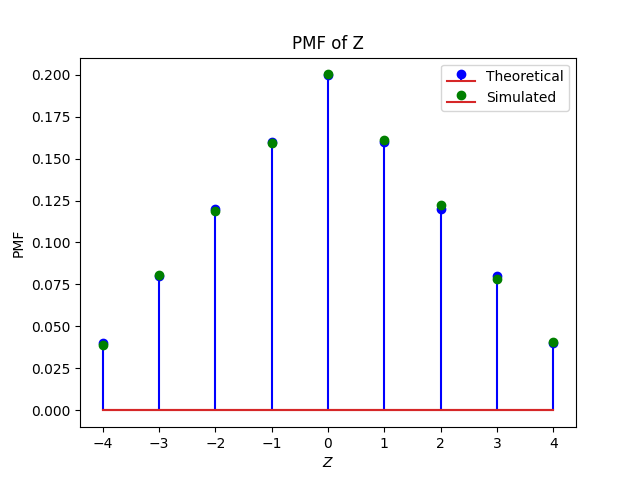
\includegraphics[width=\columnwidth]{ncert/10/15/2/1/figs/figure1.png}
\caption{PMF of $Z$}
\end{figure}
\\
The cumulative distributive function for $\abs{Z}$ is:
\begin{align}
	F_{\abs{Z}}(k) &= \pr{\abs{Z} \leq k}\\
	&= \sum_{i = -k}^{k} p_Z\brak{i}\\
	&= \begin{cases}
		0, & k < 0\\
		\frac{1}{5}, & k = 0\\
		\frac{13}{25}, & k = 1\\
		\frac{19}{25}, & k = 2\\
		\frac{23}{25}, & k = 3\\
		1, & k = 4
	\end{cases} 
\end{align}
\begin{figure}[!ht]
\centering
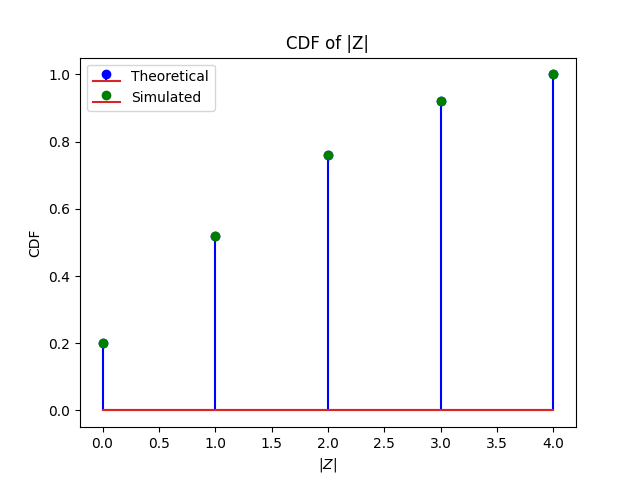
\includegraphics[width=\columnwidth]{ncert/10/15/2/1/figs/figure3.png}
\caption{CDF of $\abs{Z}$}
\end{figure}
\\

The pmf of $\abs{Z}$ is:
\begin{align}
	p_{\abs{Z}}\brak{k} &= F_{\abs{Z}}\brak{k} - F_{\abs{Z}}\brak{k-1}\\
	&= \begin{cases}
		\frac{1}{5}, & k = 0\\
		\frac{8}{25}, & k = 1\\
		\frac{6}{25}, & k = 2\\
		\frac{4}{25}, & k = 3\\
		\frac{2}{25}, & k = 4
	\end{cases}
\end{align}
\begin{figure}[!ht]
\centering
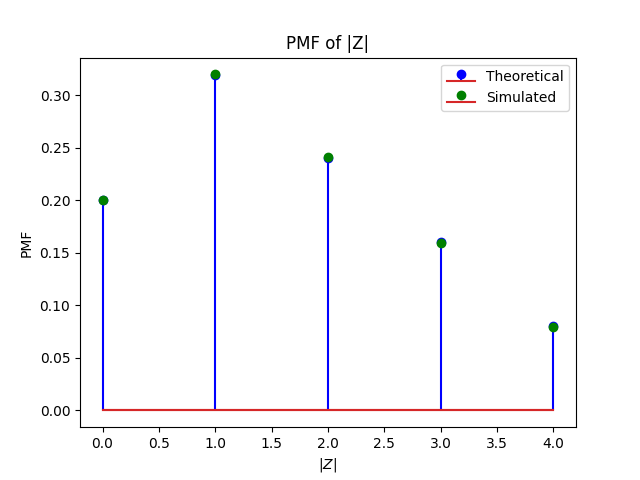
\includegraphics[width=\columnwidth]{ncert/10/15/2/1/figs/figure2.png}
\caption{PMF of $\abs{Z}$}
\end{figure}
\\
\begin{enumerate}[label=(\roman*)]
	\item the same day
	\begin{align}
	\implies X &= Y\\
	\abs{Z} &= 0\\
	p_{\abs{Z}}\brak{0} &= \frac{1}{5}
	\end{align}
	\item consecutive days
	\begin{align}
	\implies \abs{X - Y} &= 1\\
	\abs{Z} &= 1\\
	p_{\abs{Z}}\brak{1} &= \frac{8}{25}
	\end{align}
	\item different days
	\begin{align}
	\implies X &\neq Y\\
	\abs{X - Y} &\neq 0\\
	\abs{Z} &\neq 0 \\
	p_{\abs{Z}}\brak{k \neq 0} &= 1 - p_{\abs{Z}}\brak{0}\\
	&= 1 - \frac{1}{5}\\
	&= \frac{4}{5}
	\end{align}
\end{enumerate}

\begin{table}[!ht]                             
%%%%%%%%%%%%%%%%%%%%%%%%%%%%%%%%%%%%%%%%%%%%%%%%%%%%%%%%%%%%%%%%%%%%%%
%%                                                                  %%
%%  This is the header of a LaTeX2e file exported from Gnumeric.    %%
%%                                                                  %%
%%  This file can be compiled as it stands or included in another   %%
%%  LaTeX document. The table is based on the longtable package so  %%
%%  the longtable options (headers, footers...) can be set in the   %%
%%  preamble section below (see PRAMBLE).                           %%
%%                                                                  %%
%%  To include the file in another, the following two lines must be %%
%%  in the including file:                                          %%
%%        \def\inputGnumericTable{}                                 %%
%%  at the beginning of the file and:                               %%
%%        \input{name-of-this-file.tex}                             %%
%%  where the table is to be placed. Note also that the including   %%
%%  file must use the following packages for the table to be        %%
%%  rendered correctly:                                             %%
%%    \usepackage[latin1]{inputenc}                                 %%
%%    \usepackage{color}                                            %%
%%    \usepackage{array}                                            %%
%%    \usepackage{longtable}                                        %%
%%    \usepackage{calc}                                             %%
%%    \usepackage{multirow}                                         %%
%%    \usepackage{hhline}                                           %%
%%    \usepackage{ifthen}                                           %%
%%  optionally (for landscape tables embedded in another document): %%
%%    \usepackage{lscape}                                           %%
%%                                                                  %%
%%%%%%%%%%%%%%%%%%%%%%%%%%%%%%%%%%%%%%%%%%%%%%%%%%%%%%%%%%%%%%%%%%%%%%



%%  This section checks if we are begin input into another file or  %%
%%  the file will be compiled alone. First use a macro taken from   %%
%%  the TeXbook ex 7.7 (suggestion of Han-Wen Nienhuys).            %%
\def\ifundefined#1{\expandafter\ifx\csname#1\endcsname\relax}


%%  Check for the \def token for inputed files. If it is not        %%
%%  defined, the file will be processed as a standalone and the     %%
%%  preamble will be used.                                          %%
\ifundefined{inputGnumericTable}

%%  We must be able to close or not the document at the end.        %%
	\def\gnumericTableEnd{\end{document}}


%%%%%%%%%%%%%%%%%%%%%%%%%%%%%%%%%%%%%%%%%%%%%%%%%%%%%%%%%%%%%%%%%%%%%%
%%                                                                  %%
%%  This is the PREAMBLE. Change these values to get the right      %%
%%  paper size and other niceties.                                  %%
%%                                                                  %%
%%%%%%%%%%%%%%%%%%%%%%%%%%%%%%%%%%%%%%%%%%%%%%%%%%%%%%%%%%%%%%%%%%%%%%

	\documentclass[12pt%
			  %,landscape%
                    ]{report}
       \usepackage[latin1]{inputenc}
       \usepackage{fullpage}
       \usepackage{color}
       \usepackage{array}
       \usepackage{longtable}
       \usepackage{calc}
       \usepackage{multirow}
       \usepackage{hhline}
       \usepackage{ifthen}

	\begin{document}


%%  End of the preamble for the standalone. The next section is for %%
%%  documents which are included into other LaTeX2e files.          %%
\else

%%  We are not a stand alone document. For a regular table, we will %%
%%  have no preamble and only define the closing to mean nothing.   %%
    \def\gnumericTableEnd{}

%%  If we want landscape mode in an embedded document, comment out  %%
%%  the line above and uncomment the two below. The table will      %%
%%  begin on a new page and run in landscape mode.                  %%
%       \def\gnumericTableEnd{\end{landscape}}
%       \begin{landscape}


%%  End of the else clause for this file being \input.              %%
\fi

%%%%%%%%%%%%%%%%%%%%%%%%%%%%%%%%%%%%%%%%%%%%%%%%%%%%%%%%%%%%%%%%%%%%%%
%%                                                                  %%
%%  The rest is the gnumeric table, except for the closing          %%
%%  statement. Changes below will alter the table's appearance.     %%
%%                                                                  %%
%%%%%%%%%%%%%%%%%%%%%%%%%%%%%%%%%%%%%%%%%%%%%%%%%%%%%%%%%%%%%%%%%%%%%%

\providecommand{\gnumericmathit}[1]{#1} 
%%  Uncomment the next line if you would like your numbers to be in %%
%%  italics if they are italizised in the gnumeric table.           %%
%\renewcommand{\gnumericmathit}[1]{\mathit{#1}}
\providecommand{\gnumericPB}[1]%
{\let\gnumericTemp=\\#1\let\\=\gnumericTemp\hspace{0pt}}
 \ifundefined{gnumericTableWidthDefined}
        \newlength{\gnumericTableWidth}
        \newlength{\gnumericTableWidthComplete}
        \newlength{\gnumericMultiRowLength}
        \global\def\gnumericTableWidthDefined{}
 \fi
%% The following setting protects this code from babel shorthands.  %%
 \ifthenelse{\isundefined{\languageshorthands}}{}{\languageshorthands{english}}
%%  The default table format retains the relative column widths of  %%
%%  gnumeric. They can easily be changed to c, r or l. In that case %%
%%  you may want to comment out the next line and uncomment the one %%
%%  thereafter                                                      %%
\providecommand\gnumbox{\makebox[0pt]}
%%\providecommand\gnumbox[1][]{\makebox}

%% to adjust positions in multirow situations                       %%
\setlength{\bigstrutjot}{\jot}
\setlength{\extrarowheight}{\doublerulesep}

%%  The \setlongtables command keeps column widths the same across  %%
%%  pages. Simply comment out next line for varying column widths.  %%
\setlongtables

\setlength\gnumericTableWidth{%
	75pt+%
	75pt+%
	75pt+%
0pt}
\def\gumericNumCols{3}
\setlength\gnumericTableWidthComplete{\gnumericTableWidth+%
         \tabcolsep*\gumericNumCols*2+\arrayrulewidth*\gumericNumCols}
\ifthenelse{\lengthtest{\gnumericTableWidthComplete > \linewidth}}%
         {\def\gnumericScale{1*\ratio{\linewidth-%
                        \tabcolsep*\gumericNumCols*2-%
                        \arrayrulewidth*\gumericNumCols}%
{\gnumericTableWidth}}}%
{\def\gnumericScale{1}}

%%%%%%%%%%%%%%%%%%%%%%%%%%%%%%%%%%%%%%%%%%%%%%%%%%%%%%%%%%%%%%%%%%%%%%
%%                                                                  %%
%% The following are the widths of the various columns. We are      %%
%% defining them here because then they are easier to change.       %%
%% Depending on the cell formats we may use them more than once.    %%
%%                                                                  %%
%%%%%%%%%%%%%%%%%%%%%%%%%%%%%%%%%%%%%%%%%%%%%%%%%%%%%%%%%%%%%%%%%%%%%%

\ifthenelse{\isundefined{\gnumericColA}}{\newlength{\gnumericColA}}{}\settowidth{\gnumericColA}{\begin{tabular}{@{}p{75pt*\gnumericScale}@{}}x\end{tabular}}
\ifthenelse{\isundefined{\gnumericColB}}{\newlength{\gnumericColB}}{}\settowidth{\gnumericColB}{\begin{tabular}{@{}p{100pt*\gnumericScale}@{}}x\end{tabular}}
\ifthenelse{\isundefined{\gnumericColC}}{\newlength{\gnumericColC}}{}\settowidth{\gnumericColC}{\begin{tabular}{@{}p{200pt*\gnumericScale}@{}}x\end{tabular}}

%\begin{longtable}[c]{%
\begin{tabular}[c]{%
	b{\gnumericColA}%
	b{\gnumericColB}%
	b{\gnumericColC}%
	}

\hhline{|-|-|-|}
	 \multicolumn{1}{|p{\gnumericColA}|}%
	{\gnumericPB{\raggedright}\gnumbox[l]{\textbf{parameter}}}
	&\multicolumn{1}{p{\gnumericColB}|}%
	{\gnumericPB{\raggedright}\gnumbox[l]{\textbf{value}}}
	&\multicolumn{1}{p{\gnumericColC}|}%
	{\gnumericPB{\raggedright}\gnumbox[l]{\textbf{description}}}

\\
\hhline{|---|}
	 \multicolumn{1}{|p{\gnumericColA}|}%
	{\gnumericPB{\raggedright}\gnumbox[l]{$X$}}
	&\multicolumn{1}{p{\gnumericColB}|}%
	{\gnumericPB{\raggedright}\gnumbox[l]{$\cbrak{0,1,2,3,4}$}}
	&\multicolumn{1}{p{\gnumericColC}|}%
	{\gnumericPB{\raggedright}\gnumbox[l]{Denotes the day on which Shyam visits the shop}}
\\
\hhline{|---|}
	 \multicolumn{1}{|p{\gnumericColA}|}%
	{\gnumericPB{\raggedright}\gnumbox[l]{$Y$}}
	&\multicolumn{1}{p{\gnumericColB}|}%
	{\gnumericPB{\raggedright}\gnumbox[l]{$\cbrak{0,1,2,3,4}$}}
	&\multicolumn{1}{p{\gnumericColC}|}%
	{\gnumericPB{\raggedright}\gnumbox[l]{Denotes the day on which Ekta visits the shop}}
\\
\hhline{|---|}
	 \multicolumn{1}{|p{\gnumericColA}|}%
	{\gnumericPB{\raggedright}\gnumbox[l]{$Z$}}
	&\multicolumn{1}{p{\gnumericColB}|}%
	{\gnumericPB{\raggedright}\gnumbox[l]{$\cbrak{-4,-3,-2,-1,0,1,2,3,4}$}}
	&\multicolumn{1}{p{\gnumericColC}|}%
	{\gnumericPB{\raggedright}\gnumbox[l]{$X - Y$}}
\\

\hhline{|-|-|-|}
%\end{longtable}
\end{tabular}

\ifthenelse{\isundefined{\languageshorthands}}{}{\languageshorthands{\languagename}}
\gnumericTableEnd
  
\caption{Random Variables}
\end{table}





\item Let X represent the difference between the number of heads and the number of tails obtained when a coin is tossed 6 times. What are the possible values of X? Also find the Probability distribution of X.
\\
       \iffalse
\let\negmedspace\undefined
\let\negthickspace\undefined
\documentclass[journal,12pt,onecolumn]{IEEEtran}
\usepackage{cite}
\usepackage{amsmath,amssymb,amsfonts,amsthm}
\usepackage{algorithmic}
\usepackage{graphicx}
\usepackage{textcomp}
\usepackage{xcolor}
\usepackage{txfonts}
\usepackage{listings}
\usepackage{enumitem}
\usepackage{mathtools}
\usepackage{gensymb}
\usepackage[breaklinks=true]{hyperref}
\usepackage{tkz-euclide} % loads  TikZ and tkz-base
\usepackage{listings}
\usepackage{gvv}
%
%\usepackage{setspace}
%\usepackage{gensymb}
%\doublespacing
%\singlespacing

%\usepackage{graphicx}
%\usepackage{amssymb}
%\usepackage{relsize}
%\usepackage[cmex10]{amsmath}
%\usepackage{amsthm}
%\interdisplaylinepenalty=2500
%\savesymbol{iint}
%\usepackage{txfonts}
%\restoresymbol{TXF}{iint}
%\usepackage{wasysym}
%\usepackage{amsthm}
%\usepackage{iithtlc}
%\usepackage{mathrsfs}
%\usepackage{txfonts}
%\usepackage{stfloats}
%\usepackage{bm}
%\usepackage{cite}
%\usepackage{cases}
%\usepackage{subfig}
%\usepackage{xtab}
%\usepackage{longtable}
%\usepackage{multirow}
%\usepackage{algorithm}
%\usepackage{algpseudocode}
%\usepackage{enumitem}
%\usepackage{mathtools}
%\usepackage{tikz}
%\usepackage{circuitikz}
%\usepackage{verbatim}
%\usepackage{tfrupee}
%\usepackage{stmaryrd}
%\usetkzobj{all}
%    \usepackage{color}                                            %%
%    \usepackage{array}                                            %%
%    \usepackage{longtable}                                        %%
%    \usepackage{calc}                                             %%
%    \usepackage{multirow}                                         %%
%    \usepackage{hhline}                                           %%
%    \usepackage{ifthen}                                           %%
  %optionally (for landscape tables embedded in another document): %%
%    \usepackage{lscape}     
%\usepackage{multicol}
%\usepackage{chngcntr}
%\usepackage{enumerate}

%\usepackage{wasysym}
%\documentclass[conference]{IEEEtran}
%\IEEEoverridecommandlockouts
% The preceding line is only needed to identify funding in the first footnote. If that is unneeded, please comment it out.

\newtheorem{theorem}{Theorem}[section]
\newtheorem{problem}{Problem}
\newtheorem{proposition}{Proposition}[section]
\newtheorem{lemma}{Lemma}[section]
\newtheorem{corollary}[theorem]{Corollary}
\newtheorem{example}{Example}[section]
\newtheorem{definition}[problem]{Definition}
%\newtheorem{thm}{Theorem}[section] 
%\newtheorem{defn}[thm]{Definition}
%\newtheorem{algorithm}{Algorithm}[section]
%\newtheorem{cor}{Corollary}
\newcommand{\BEQA}{\begin{eqnarray}}
\newcommand{\EEQA}{\end{eqnarray}}
\newcommand{\define}{\stackrel{\triangle}{=}}
\theoremstyle{remark}
\newtheorem{rem}{Remark}

%\bibliographystyle{ieeetr}
\begin{document}
\parindent 0px

\bibliographystyle{IEEEtran}


\vspace{3cm}

\title{
%	\logo{
Solution to 12.13.4.3
%	}
}
\author{ Aryan Jain - EE22BTECH11011$^{*}$% <-this % stops a space	
}	
%\title{
%	\logo{Matrix Analysis through Octave}{\begin{center}\includegraphics[scale=.24]{tlc}\end{center}}{}{HAMDSP}
%}


% paper title
% can use linebreaks \\ within to get better formatting as desired
%\title{Matrix Analysis through Octave}
%
%
% author names and IEEE memberships
% note positions of commas and nonbreaking spaces ( ~ ) LaTeX will not break
% a structure at a ~ so this keeps an author's name from being broken across
% two lines.
% use \thanks{} to gain access to the first footnote area
% a separate \thanks must be used for each paragraph as LaTeX2e's \thanks
% was not built to handle multiple paragraphs
%

%\author{<-this % stops a space
%\thanks{}}
%}
% note the % following the last \IEEEmembership and also \thanks - 
% these prevent an unwanted space from occurring between the last author name
% and the end of the author line. i.e., if you had this:
% 
% \author{....lastname \thanks{...} \thanks{...} }
%                     ^------------^------------^----Do not want these spaces!
%
% a space would be appended to the last name and could cause every name on that
% line to be shifted left slightly. This is one of those "LaTeX things". For
% instance, "\textbf{A} \textbf{B}" will typeset as "A B" not "AB". To get
% "AB" then you have to do: "\textbf{A}\textbf{B}"
% \thanks is no different in this regard, so shield the last } of each \thanks
% that ends a line with a % and do not let a space in before the next \thanks.
% Spaces after \IEEEmembership other than the last one are OK (and needed) as
% you are supposed to have spaces between the names. For what it is worth,
% this is a minor point as most people would not even notice if the said evil
% space somehow managed to creep in.



% The paper headers
%\markboth{Journal of \LaTeX\ Class Files,~Vol.~6, No.~1, January~2007}%
%{Shell \MakeLowercase{\textit{et al.}}: Bare Demo of IEEEtran.cls for Journals}
% The only time the second header will appear is for the odd numbered pages
% after the title page when using the twoside option.
% 
% *** Note that you probably will NOT want to include the author's ***
% *** name in the headers of peer review papers.                   ***
% You can use \ifCLASSOPTIONpeerreview for conditional compilation here if
% you desire.




% If you want to put a publisher's ID mark on the page you can do it like
% this:
%\IEEEpubid{0000--0000/00\$00.00~\copyright~2007 IEEE}
% Remember, if you use this you must call \IEEEpubidadjcol in the second
% column for its text to clear the IEEEpubid mark.



% make the title area
\maketitle



%\tableofcontents

\bigskip

\renewcommand{\thefigure}{\theenumi}
\renewcommand{\thetable}{\theenumi}
%\renewcommand{\theequation}{\theenumi}

%\begin{abstract}
%%\boldmath
%In this letter, an algorithm for evaluating the exact analytical bit error rate  (BER)  for the piecewise linear (PL) combiner for  multiple relays is presented. Previous results were available only for upto three relays. The algorithm is unique in the sense that  the actual mathematical expressions, that are prohibitively large, need not be explicitly obtained. The diversity gain due to multiple relays is shown through plots of the analytical BER, well supported by simulations. 
%
%\end{abstract}
% IEEEtran.cls defaults to using nonbold math in the Abstract.
% This preserves the distinction between vectors and scalars. However,
% if the journal you are submitting to favors bold math in the abstract,
% then you can use LaTeX's standard command \boldmath at the very start
% of the abstract to achieve this. Many IEEE journals frown on math
% in the abstract anyway.

% Note that keywords are not normally used for peerreview papers.
%\begin{IEEEkeywords}
%Cooperative diversity, decode and forward, piecewise linear
%\end{IEEEkeywords}



% For peer review papers, you can put extra information on the cover
% page as needed:
% \ifCLASSOPTIONpeerreview
% \begin{center} \bfseries EDICS Category: 3-BBND \end{center}
% \fi
%
% For peerreview papers, this IEEEtran command inserts a page break and
% creates the second title. It will be ignored for other modes.
%\IEEEpeerreviewmaketitle
\textbf{Question}:
Let X represent the difference between the number of heads and the number of tails obtained when a coin is tossed 6 times. What are the possible values of X? Also find the Probability distribution of X.
\newline
\fi
\solution
\newline
It is given that the coin is tossed 6 times.
\newline
Let $H$ be a random variable which denotes the number of heads,
\begin{align}
      H = \{0,1,2,3,4,5,6\}
\end{align}
Let $T$ be a random variable which denotes the number of tails,
\begin{align}
      T &= 6 - H \\
        &= \{6,5,4,3,2,1,0\}
\end{align}
Let X be a random variable which denotes the absolute value of the difference between the number of heads and number of tails,
\begin{align}  
      X &= |H - T| \\
        &= |H - (6 - H)| \\
        &= |2H - 6| 
\end{align} 
Therefore, X can take values from the set \{0,2,4,6\}.  
\newline
Now we will find the probability distribution of X using the CDF approach,
\newline
The CDF of H is given by:
\begin{align}
F_H(k) &= \pr{H \leq k} \\
       &=   \sum_{i=0}^{k} \pr{H=i} \\ 
       &=   \sum_{i=0}^{k} \frac{\comb{6}{i}}{2^6}
\end{align}
First we will do the analysis for k = 2,4 and 6
\newline
So the CDF of X will be:
\begin{align}
F_X(k) &= \pr{X \leq k} \\
       &= \pr{|2H-6| \leq k} \\
       &= \pr{-k \leq 2H-6 \leq k} \\
       &= \pr{\frac{6-k}{2} \leq H \leq \frac{6+k}{2}} \\
       &= F_H\brak{3+\frac{k}{2}} - F_H\brak{(3-\frac{k}{2})-1} \\
       &= F_H\brak{3+\frac{k}{2}} - F_H\brak{2-\frac{k}{2}}
\end{align}
So the probability distribution of X would be given by:
\begin{align}
p_X(k) &= F_X(k) - F_X(k-1) \\
       &= F_H\brak{3+\frac{k}{2}} - F_H\brak{2-\frac{k}{2}} - F_H\brak{2.5+\frac{k}{2}} + F_H\brak{3.5-\frac{k}{2}} \\
       &= \brak{\sum_{i=0}^{3+\frac{k}{2}} \frac{\comb{6}{i}}{2^6} - \sum_{i=0}^{2.5+\frac{k}{2}} \frac{\comb{6}{i}}{2^6}} + \brak{\sum_{i=0}^{3.5-\frac{k}{2}} \frac{\comb{6}{i}}{2^6} - \sum_{i=0}^{2-\frac{k}{2}} \frac{\comb{6}{i}}{2^6}} \\
       &= \frac{\comb{6}{k}}{2^6} + \frac{\comb{6}{6-k}}{2^6} \\
       &= \frac{\comb{6}{k}}{2^5}   \quad \brak{k = 2,4,6}
\end{align}
Now we will do the analysis for k = 0,
\newline
CDF of X for will be
\begin{align}
F_X(k) &= F_H\brak{\sbrak{3+\frac{k}{2}}} - F_H\brak{\sbrak{3-\frac{k}{2}}}
\end{align}
So the probability distribution of X would be given by:
\begin{align}
p_X(k) &= F_X(k) - F_X(k-1) \\
       &= F_H\brak{\sbrak{3+\frac{k}{2}}} - F_H\brak{\sbrak{3-\frac{k}{2}}} - F_H\brak{\sbrak{2.5+\frac{k}{2}}} + F_H\brak{\sbrak{3.5-\frac{k}{2}}} \\
       &= F_H\brak{3+\sbrak{\frac{k}{2}}} - F_H\brak{3-\sbrak{\frac{k}{2}}} - F_H\brak{2+\sbrak{\frac{k}{2}}} + F_H\brak{3-\sbrak{\frac{k}{2}}} \\
       &= F_H\brak{3+\sbrak{\frac{k}{2}}} - F_H\brak{2+\sbrak{\frac{k}{2}}} \\
       &= \sum_{i=0}^{3+\sbrak{\frac{k}{2}}} \frac{\comb{6}{i}}{2^6} - \sum_{i=0}^{2+\sbrak{\frac{k}{2}}} \frac{\comb{6}{i}}{2^6} \quad \brak{k = 0}
\end{align}
The plot of probability distribution of X is shown below:
\begin{figure}
\centering
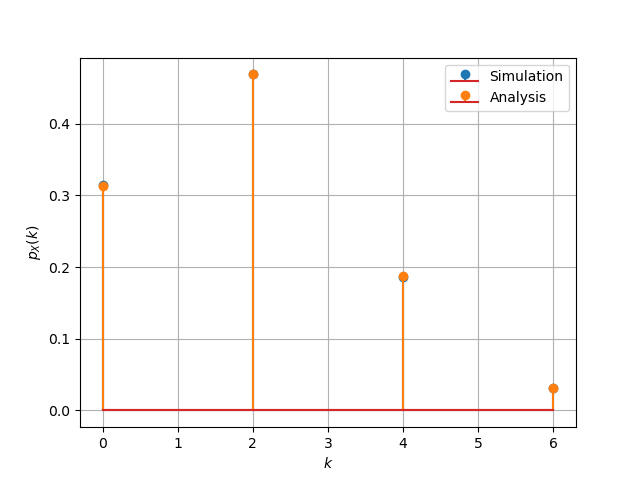
\includegraphics[width=\columnwidth]{ncert/12/13/4/3/figs/fig.png}
\caption{ PMF of $X$}
\label{Fig:1 X_pmf}
\end{figure}

\end{document}

       \item A black and a red dice are rolled.\\
(a) find the conditional probability of obtaining a sum greater than 9,given that the black dice resulted in a 5.\\
(b) find the conditional probability of obtaining the sum 8,given that the red die resulted in a number less than 4.\\
\solution
\iffalse
\documentclass[journal,12pt,twocolumn]{IEEEtran}
\usepackage{setspace}
\usepackage{gensymb}
\singlespacing
\usepackage[cmex10]{amsmath}
\usepackage{amsthm}
\usepackage{mathrsfs}
\usepackage{txfonts}
\usepackage{stfloats}
\usepackage{bm}
\usepackage{cite}
\usepackage{cases}
\usepackage{subfig}
\usepackage{longtable}
\usepackage{multirow}
\usepackage{enumitem}
\usepackage{mathtools}
\usepackage{tikz}
\usepackage{circuitikz}
\usepackage{verbatim}
\usepackage[breaklinks=true]{hyperref}
\usepackage{tkz-euclide} % loads  TikZ and tkz-base
\usepackage{listings}
\usepackage{color}    
\usepackage{array}    
\usepackage{longtable}
\usepackage{calc}     
\usepackage{multirow} 
\usepackage{hhline}   
\usepackage{ifthen}   
\usepackage{lscape}     
\usepackage{chngcntr}
\usepackage{float}
\DeclareMathOperator*{\Res}{Res}
\renewcommand\thesection{\arabic{section}}
\renewcommand\thesubsection{\thesection.\arabic{subsection}}
\renewcommand\thesubsubsection{\thesubsection.\arabic{subsubsection}}

\renewcommand\thesectiondis{\arabic{section}}
\renewcommand\thesubsectiondis{\thesectiondis.\arabic{subsection}}
\renewcommand\thesubsubsectiondis{\thesubsectiondis.\arabic{subsubsection}}
\renewcommand\thetable{\arabic{table}}
% correct bad hyphenation here
\hyphenation{op-tical net-works semi-conduc-tor}
\def\inputGnumericTable{}                                 %%

\lstset{
%language=C,
frame=single, 
breaklines=true,
columns=fullflexible
}
%\lstset{
%language=tex,
%frame=single, 
%breaklines=true
%}

\begin{document}
\newtheorem{theorem}{Theorem}[section]
\newtheorem{problem}{Problem}
\newtheorem{proposition}{Proposition}[section]
\newtheorem{lemma}{Lemma}[section]
\newtheorem{corollary}[theorem]{Corollary}
\newtheorem{example}{Example}[section]
\newtheorem{definition}[problem]{Definition}
\newcommand{\BEQA}{\begin{eqnarray}}
\newcommand{\EEQA}{\end{eqnarray}}
\newcommand{\define}{\stackrel{\triangle}{=}}
\bibliographystyle{IEEEtran}
\providecommand{\mbf}{\mathbf}
\providecommand{\pr}[1]{\ensuremath{\Pr\left(#1\right)}}
\providecommand{\qfunc}[1]{\ensuremath{Q\left(#1\right)}}
\providecommand{\sbrak}[1]{\ensuremath{{}\left[#1\right]}}
\providecommand{\lsbrak}[1]{\ensuremath{{}\left[#1\right.}}
\providecommand{\rsbrak}[1]{\ensuremath{{}\left.#1\right]}}
\providecommand{\brak}[1]{\ensuremath{\left(#1\right)}}
\providecommand{\lbrak}[1]{\ensuremath{\left(#1\right.}}
\providecommand{\rbrak}[1]{\ensuremath{\left.#1\right)}}
\providecommand{\cbrak}[1]{\ensuremath{\left\{#1\right\}}}
\providecommand{\lcbrak}[1]{\ensuremath{\left\{#1\right.}}
\providecommand{\rcbrak}[1]{\ensuremath{\left.#1\right\}}}
\theoremstyle{remark}
\newtheorem{rem}{Remark}
\newcommand{\sgn}{\mathop{\mathrm{sgn}}}
\providecommand{\abs}[1]{\left\vert#1\right\vert}
\providecommand{\res}[1]{\Res\displaylimits_{#1}} 
\providecommand{\norm}[1]{\left\lVert#1\right\rVert}
\providecommand{\mtx}[1]{\mathbf{#1}}
\providecommand{\mean}[1]{E\left[ #1 \right]}
\providecommand{\fourier}{\overset{\mathcal{F}}{ \rightleftharpoons}}
\providecommand{\system}[1]{\overset{\mathcal{#1}}{ \longleftrightarrow}}
\newcommand{\solution}{\noindent \textbf{Solution: }}
\newcommand{\cosec}{\,\text{cosec}\,}
\providecommand{\dec}[2]{\ensuremath{\overset{#1}{\underset{#2}{\gtrless}}}}
\newcommand{\myvec}[1]{\ensuremath{\begin{pmatrix}#1\end{pmatrix}}}
\newcommand{\mydet}[1]{\ensuremath{\begin{vmatrix}#1\end{vmatrix}}}
\let\vec\mathbf
\def\putbox#1#2#3{\makebox[0in][l]{\makebox[#1][l]{}\raisebox{\baselineskip}[0in][0in]{\raisebox{#2}[0in][0in]{#3}}}}
     \def\rightbox#1{\makebox[0in][r]{#1}}
     \def\centbox#1{\makebox[0in]{#1}}
     \def\topbox#1{\raisebox{-\baselineskip}[0in][0in]{#1}}
     \def\midbox#1{\raisebox{-0.5\baselineskip}[0in][0in]{#1}}\let\vec\mathbf


\bibliographystyle{IEEEtran}


\vspace{3cm}

\title{Problem}

\author{EE22BTECH11010 - Aryan Bubna
}	
%\title{
%	\logo{Matrix Analysis through Octave}{\begin{center}\includegraphics[scale=.24]{tlc}\end{center}}{}{HAMDSP}
%}


% paper title
% can use linebreaks \\ within to get better formatting as desired
%\title{Matrix Analysis through Octave}
%
%
% author names and IEEE memberships
% note positions of commas and nonbreaking spaces ( ~ ) LaTeX will not break
% a structure at a ~ so this keeps an author's name from being broken across
% two lines.
% use \thanks{} to gain access to the first footnote area
% a separate \thanks must be used for each paragraph as LaTeX2e's \thanks
% was not built to handle multiple paragraphs
%

%\author{<-this % stops a space
%\thanks{}}
%}
% note the % following the last \IEEEmembership and also \thanks - 
% these prevent an unwanted space from occurring between the last author name
% and the end of the author line. i.e., if you had this:
% 
% \author{....lastname \thanks{...} \thanks{...} }
%                     ^------------^------------^----Do not want these spaces!
%
% a space would be appended to the last name and could cause every name on that
% line to be shifted left slightly. This is one of those "LaTeX things". For
% instance, "\textbf{A} \textbf{B}" will typeset as "A B" not "AB". To get
% "AB" then you have to do: "\textbf{A}\textbf{B}"
% \thanks is no different in this regard, so shield the last } of each \thanks
% that ends a line with a % and do not let a space in before the next \thanks.
% Spaces after \IEEEmembership other than the last one are OK (and needed) as
% you are supposed to have spaces between the names. For what it is worth,
% this is a minor point as most people would not even notice if the said evil
% space somehow managed to creep in.



% The paper headers
%\markboth{Journal of \LaTeX\ Class Files,~Vol.~6, No.~1, January~2007}%
%{Shell \MakeLowercase{\textit{et al.}}: Bare Demo of IEEEtran.cls for Journals}
% The only time the second header will appear is for the odd numbered pages
% after the title page when using the twoside option.
% 
% *** Note that you probably will NOT want to include the author's ***
% *** name in the headers of peer review papers.                   ***
% You can use \ifCLASSOPTIONpeerreview for conditional compilation here if
% you desire.




% If you want to put a publisher's ID mark on the page you can do it like
% this:
%\IEEEpubid{0000--0000/00\$00.00~\copyright~2007 IEEE}
% Remember, if you use this you must call \IEEEpubidadjcol in the second
% column for its text to clear the IEEEpubid mark.



% make the title area
\maketitle

\newpage

%\tableofcontents

\bigskip

\renewcommand{\thefigure}{\theenumi}
\renewcommand{\thetable}{\theenumi}
question: A black and a red dice are rolled.

(a) find the conditional probability of obtaining a sum greater than 9,given that the black dice resulted in a 5.

(b) find the conditional probability of obtaining the sum 8,given that the red die resulted in a number less than 4.

\solution
\fi
\begin{table}[!ht]
%%%%%%%%%%%%%%%%%%%%%%%%%%%%%%%%%%%%%%%%%%%%%%%%%%%%%%%%%%%%%%%%%%%%%%
%%                                                                  %%
%%  This is the header of a LaTeX2e file exported from Gnumeric.    %%
%%                                                                  %%
%%  This file can be compiled as it stands or included in another   %%
%%  LaTeX document. The table is based on the longtable package so  %%
%%  the longtable options (headers, footers...) can be set in the   %%
%%  preamble section below (see PRAMBLE).                           %%
%%                                                                  %%
%%  To include the file in another, the following two lines must be %%
%%  in the including file:                                          %%
%%        \def\inputGnumericTable{}                                 %%
%%  at the beginning of the file and:                               %%
%%        \input{name-of-this-file.tex}                             %%
%%  where the table is to be placed. Note also that the including   %%
%%  file must use the following packages for the table to be        %%
%%  rendered correctly:                                             %%
%%    \usepackage[latin1]{inputenc}                                 %%
%%    \usepackage{color}                                            %%
%%    \usepackage{array}                                            %%
%%    \usepackage{longtable}                                        %%
%%    \usepackage{calc}                                             %%
%%    \usepackage{multirow}                                         %%
%%    \usepackage{hhline}                                           %%
%%    \usepackage{ifthen}                                           %%
%%  optionally (for landscape tables embedded in another document): %%
%%    \usepackage{lscape}                                           %%
%%                                                                  %%
%%%%%%%%%%%%%%%%%%%%%%%%%%%%%%%%%%%%%%%%%%%%%%%%%%%%%%%%%%%%%%%%%%%%%%



%%  This section checks if we are begin input into another file or  %%
%%  the file will be compiled alone. First use a macro taken from   %%
%%  the TeXbook ex 7.7 (suggestion of Han-Wen Nienhuys).            %%
\def\ifundefined#1{\expandafter\ifx\csname#1\endcsname\relax}


%%  Check for the \def token for inputed files. If it is not        %%
%%  defined, the file will be processed as a standalone and the     %%
%%  preamble will be used.                                          %%
\ifundefined{inputGnumericTable}

%%  We must be able to close or not the document at the end.        %%
	\def\gnumericTableEnd{\end{document}}


%%%%%%%%%%%%%%%%%%%%%%%%%%%%%%%%%%%%%%%%%%%%%%%%%%%%%%%%%%%%%%%%%%%%%%
%%                                                                  %%
%%  This is the PREAMBLE. Change these values to get the right      %%
%%  paper size and other niceties.                                  %%
%%                                                                  %%
%%%%%%%%%%%%%%%%%%%%%%%%%%%%%%%%%%%%%%%%%%%%%%%%%%%%%%%%%%%%%%%%%%%%%%

	\documentclass[12pt%
			  %,landscape%
                    ]{report}
       \usepackage[latin1]{inputenc}
       \usepackage{fullpage}
       \usepackage{color}
       \usepackage{array}
       \usepackage{longtable}
       \usepackage{calc}
       \usepackage{multirow}
       \usepackage{hhline}
       \usepackage{ifthen}

	\begin{document}


%%  End of the preamble for the standalone. The next section is for %%
%%  documents which are included into other LaTeX2e files.          %%
\else

%%  We are not a stand alone document. For a regular table, we will %%
%%  have no preamble and only define the closing to mean nothing.   %%
    \def\gnumericTableEnd{}

%%  If we want landscape mode in an embedded document, comment out  %%
%%  the line above and uncomment the two below. The table will      %%
%%  begin on a new page and run in landscape mode.                  %%
%       \def\gnumericTableEnd{\end{landscape}}
%       \begin{landscape}


%%  End of the else clause for this file being \input.              %%
\fi

%%%%%%%%%%%%%%%%%%%%%%%%%%%%%%%%%%%%%%%%%%%%%%%%%%%%%%%%%%%%%%%%%%%%%%
%%                                                                  %%
%%  The rest is the gnumeric table, except for the closing          %%
%%  statement. Changes below will alter the table's appearance.     %%
%%                                                                  %%
%%%%%%%%%%%%%%%%%%%%%%%%%%%%%%%%%%%%%%%%%%%%%%%%%%%%%%%%%%%%%%%%%%%%%%

\providecommand{\gnumericmathit}[1]{#1} 
%%  Uncomment the next line if you would like your numbers to be in %%
%%  italics if they are italizised in the gnumeric table.           %%
%\renewcommand{\gnumericmathit}[1]{\mathit{#1}}
\providecommand{\gnumericPB}[1]%
{\let\gnumericTemp=\\#1\let\\=\gnumericTemp\hspace{0pt}}
 \ifundefined{gnumericTableWidthDefined}
        \newlength{\gnumericTableWidth}
        \newlength{\gnumericTableWidthComplete}
        \newlength{\gnumericMultiRowLength}
        \global\def\gnumericTableWidthDefined{}
 \fi
%% The following setting protects this code from babel shorthands.  %%
 \ifthenelse{\isundefined{\languageshorthands}}{}{\languageshorthands{english}}
%%  The default table format retains the relative column widths of  %%
%%  gnumeric. They can easily be changed to c, r or l. In that case %%
%%  you may want to comment out the next line and uncomment the one %%
%%  thereafter                                                      %%
\providecommand\gnumbox{\makebox[0pt]}
%%\providecommand\gnumbox[1][]{\makebox}

%% to adjust positions in multirow situations                       %%
\setlength{\bigstrutjot}{\jot}
\setlength{\extrarowheight}{\doublerulesep}

%%  The \setlongtables command keeps column widths the same across  %%
%%  pages. Simply comment out next line for varying column widths.  %%
\setlongtables

\setlength\gnumericTableWidth{%
	53pt+%
	53pt+%
	53pt+%
0pt}
\def\gumericNumCols{3}
\setlength\gnumericTableWidthComplete{\gnumericTableWidth+%
         \tabcolsep*\gumericNumCols*2+\arrayrulewidth*\gumericNumCols}
\ifthenelse{\lengthtest{\gnumericTableWidthComplete > \linewidth}}%
         {\def\gnumericScale{1*\ratio{\linewidth-%
                        \tabcolsep*\gumericNumCols*2-%
                        \arrayrulewidth*\gumericNumCols}%
{\gnumericTableWidth}}}%
{\def\gnumericScale{1}}

%%%%%%%%%%%%%%%%%%%%%%%%%%%%%%%%%%%%%%%%%%%%%%%%%%%%%%%%%%%%%%%%%%%%%%
%%                                                                  %%
%% The following are the widths of the various columns. We are      %%
%% defining them here because then they are easier to change.       %%
%% Depending on the cell formats we may use them more than once.    %%
%%                                                                  %%
%%%%%%%%%%%%%%%%%%%%%%%%%%%%%%%%%%%%%%%%%%%%%%%%%%%%%%%%%%%%%%%%%%%%%%

\ifthenelse{\isundefined{\gnumericColA}}{\newlength{\gnumericColA}}{}\settowidth{\gnumericColA}{\begin{tabular}{@{}p{53pt*\gnumericScale}@{}}x\end{tabular}}
\ifthenelse{\isundefined{\gnumericColB}}{\newlength{\gnumericColB}}{}\settowidth{\gnumericColB}{\begin{tabular}{@{}p{53pt*\gnumericScale}@{}}x\end{tabular}}
\ifthenelse{\isundefined{\gnumericColC}}{\newlength{\gnumericColC}}{}\settowidth{\gnumericColC}{\begin{tabular}{@{}p{53pt*\gnumericScale}@{}}x\end{tabular}}

\begin{tabular}[c]{%
	b{\gnumericColA}%
	b{\gnumericColB}%
	b{\gnumericColC}%
	}

%%%%%%%%%%%%%%%%%%%%%%%%%%%%%%%%%%%%%%%%%%%%%%%%%%%%%%%%%%%%%%%%%%%%%%
%%  The longtable options. (Caption, headers... see Goosens, p.124) %%
%	\caption{The Table Caption.}             \\	%
% \hline	% Across the top of the table.
%%  The rest of these options are table rows which are placed on    %%
%%  the first, last or every page. Use \multicolumn if you want.    %%

%%  Header for the first page.                                      %%
%	\multicolumn{3}{c}{The First Header} \\ \hline 
%	\multicolumn{1}{c}{colTag}	%Column 1
%	&\multicolumn{1}{c}{colTag}	%Column 2
%	&\multicolumn{1}{c}{colTag}	\\ \hline %Last column
%	\endfirsthead

%%  The running header definition.                                  %%
%	\hline
%	\multicolumn{3}{l}{\ldots\small\slshape continued} \\ \hline
%	\multicolumn{1}{c}{colTag}	%Column 1
%	&\multicolumn{1}{c}{colTag}	%Column 2
%	&\multicolumn{1}{c}{colTag}	\\ \hline %Last column
%	\endhead

%%  The running footer definition.                                  %%
%	\hline
%	\multicolumn{3}{r}{\small\slshape continued\ldots} \\
%	\endfoot

%%  The ending footer definition.                                   %%
%	\multicolumn{3}{c}{That's all folks} \\ \hline 
%	\endlastfoot
%%%%%%%%%%%%%%%%%%%%%%%%%%%%%%%%%%%%%%%%%%%%%%%%%%%%%%%%%%%%%%%%%%%%%%
\hhline{|-|--}
	 \multicolumn{1}{|p{\gnumericColA}|}%
	{\gnumericPB{\raggedright}\gnumbox[l]{RV}}
	&\multicolumn{2}{p{	\gnumericColB+%
	\gnumericColC+%
	\tabcolsep*2*1}|}%
	{\gnumericPB{\centering}\gnumbox{description}}
\\

\hhline{|-|--}
	 \multicolumn{1}{|p{\gnumericColA}|}%
	{\gnumericPB{\raggedright}\gnumbox[l]{$X_1$}}
	&\multicolumn{2}{p{	\gnumericColB+%
	\gnumericColC+%
	\tabcolsep*2*1}|}%
	{\gnumericPB{\centering}\gnumbox{Black die}}
\\
\hhline{|---|}
	 \multicolumn{1}{|p{\gnumericColA}|}%
	{\gnumericPB{\raggedright}\gnumbox[l]{$X_2$}}
	&\multicolumn{2}{p{	\gnumericColB+%
	\gnumericColC+%
	\tabcolsep*2*1}|}%
	{\gnumericPB{\centering}\gnumbox{Red die}}
\\
\hhline{|-|--|}
\end{tabular}

\ifthenelse{\isundefined{\languageshorthands}}{}{\languageshorthands{\languagename}}
\gnumericTableEnd

\caption{random variables of $X_1$ and $X_2$}
\label{tab:random variables}
\end{table}

PMF of the random variables is:
\begin{align}
p_{X_j}\brak{i}&=\begin{cases}
\frac{1}{6} & j=1,2;1\leq i \leq 6
\end{cases}
\end{align}

CDF of the random variables is:
\begin{align}
F_{X_j}\brak{i}&=\begin{cases}
\frac{i}{6} & j=1,2;1\leq i \leq 6
\end{cases}
\end{align}
\begin{enumerate}
\item
\begin{align}
\pr{X_1+X_2>9 \mid X_1=5}&=\pr{X_2>4 \mid X_1=5}\\
&=\frac{\pr{X_2>4,X_1=5}}{\pr{X_1=5}}\\
&=\pr{X_2>4}\\
&=1-\pr{X_2 \le 4}\\
&=1-F_{X_2}\brak{4}\\
&=1-\frac{4}{6}\\
&=1-\frac{2}{3}\\
&=\frac{1}{3}
\end{align}
\item
\begin{align}
\pr{X_1+X_2=8|X_2<4}&=\frac{\pr{X_1+X_2=8,X_2<4}}{\pr{X_2<4}}\\
&=\frac{\sum_{i=1}^{3}p_{X_1}\brak{8-i}p_{X_2}\brak{i}}{\pr{X_2<4}}\\
&=\frac{p_{X_1}\brak{5}p_{X_2}\brak{3}+p_{X_1}\brak{6}p_{X_2}\brak{2}}{\pr{X_2<4}}\\
&=\frac{\frac{1}{36}+\frac{1}{36}}{\frac{3}{6}}\\
&=\frac{1}{9}
\end{align}
\end{enumerate}



\item A fair die is thrown two times. Let A and B be the events, 'same number each time', and a 'a total score is 10 or more', respectively. Determine whether or not A and B are independent.\\
\solution
\\
\iffalse
\let\negmedspace\undefined
\let\negthickspace\undefined
\documentclass[journal,12pt,onecolumn]{IEEEtran}
\usepackage{cite}
\usepackage{amsmath,amssymb,amsfonts,amsthm}
\usepackage{algorithmic}
\usepackage{txfonts}
\usepackage{mathtools}
\usepackage{gensymb}
\usepackage{amssymb}
\usepackage{tabularx}
\usepackage{multirow}

\DeclareMathOperator*{\Res}{Res}

\begin{document}

\newtheorem{problem}{Problem}
\newtheorem{definition}[problem]{Definition}
\newcommand{\BEQA}{\begin{eqnarray}}
\newcommand{\EEQA}{\end{eqnarray}}

\bibliographystyle{IEEEtran}

\providecommand{\mbf}{\mathbf}
\providecommand{\pr}[1]{\ensuremath{\Pr\left(#1\right)}}
\providecommand{\qfunc}[1]{\ensuremath{Q\left(#1\right)}}
\providecommand{\sbrak}[1]{\ensuremath{{}\left[#1\right]}}
\providecommand{\lsbrak}[1]{\ensuremath{{}\left[#1\right.}}
\providecommand{\rsbrak}[1]{\ensuremath{{}\left.#1\right]}}
\providecommand{\brak}[1]{\ensuremath{\left(#1\right)}}
\providecommand{\lbrak}[1]{\ensuremath{\left(#1\right.}}
\providecommand{\rbrak}[1]{\ensuremath{\left.#1\right)}}
\providecommand{\cbrak}[1]{\ensuremath{\left\{#1\right\}}}
\providecommand{\lcbrak}[1]{\ensuremath{\left\{#1\right.}}
\providecommand{\rcbrak}[1]{\ensuremath{\left.#1\right\}}}

\theoremstyle{remark}
\newtheorem{rem}{Remark}


\newcommand{\sgn}{\mathop{\mathrm{sgn}}}
\providecommand{\abs}[1]{\left\vert#1\right\vert}
\providecommand{\res}[1]{\Res\displaylimits_{#1}} 
\providecommand{\norm}[1]{\left\lVert#1\right\rVert}
%\providecommand{\norm}[1]{\lVert#1\rVert}
\providecommand{\mtx}[1]{\mathbf{#1}}
\providecommand{\mean}[1]{E\left[ #1 \right]}
\providecommand{\fourier}{\overset{\mathcal{F}}{ \rightleftharpoons}}
%\providecommand{\hilbert}{\overset{\mathcal{H}}{ \rightleftharpoons}}
\providecommand{\system}{\overset{\mathcal{H}}{ \longleftrightarrow}}
	%\newcommand{\solution}[2]{\textbf{Solution:}{#1}}
\newcommand{\solution}{\noindent \textbf{Solution: }}
\newcommand{\cosec}{\,\text{cosec}\,}
\providecommand{\dec}[2]{\ensuremath{\overset{#1}{\underset{#2}{\gtrless}}}}
\newcommand{\myvec}[1]{\ensuremath{\begin{pmatrix}#1\end{pmatrix}}}
\newcommand{\mydet}[1]{\ensuremath{\begin{vmatrix}#1\end{vmatrix}}}

\let\vec\mathbf

\vspace{3cm}

\title{
Assignment 1\\AI1110 : Probability and Random Variables
}
\author{Tumarada Padmaja\\CS22BTECH11059}

% make the title area
\maketitle
%\newpage
\bigskip
\textbf{Question:12.13.3.2:} \\
\textbf{Solution:}
\fi
See 
\tabref{tab:ncert/12/13/3/2/1}
\begin{table}[htbp]
\centering
\caption{Random Variable Declaration}
%%%%%%%%%%%%%%%%%%%%%%%%%%%%%%%%%%%%%%%%%%%%%%%%%%%%%%%%%%%%%%%%%%%%%%
%%                                                                  %%
%%  This is a LaTeX2e table fragment exported from Gnumeric.        %%
%%                                                                  %%
%%%%%%%%%%%%%%%%%%%%%%%%%%%%%%%%%%%%%%%%%%%%%%%%%%%%%%%%%%%%%%%%%%%%%%
\begin{tabular}{|c|c|c|}
\hline
Random Variable  & Value of the random variable    & Event                            \\
\hline
\multirow{2}{*}B  & 0                            & selecting first bag              \\
\cline{2-3}
                 & 1                            & selecting second bag             \\
\hline
\multirow{2}{*}R  & 0                            & choosing white ball from the bag \\
\cline{2-3}
                 & 1                            & choosing red ball from the bag   \\
\hline
\end{tabular}

\label{tab:ncert/12/13/3/2/1}
\end{table}
Given,
\begin{align}
\pr{R=1|B=0}&=\frac{4}{8}=\frac{1}{2} \\ 
\pr{R=1|B=1}&=\frac{2}{8}=\frac{1}{4} \\ 
\pr{B=0}&=\frac{1}{2} \\ 
\pr{B=1}&=\frac{1}{2} 
\end{align}
\begin{align}
\pr{B=0|R=1} &= \frac{\pr{R=1|B=0} \pr{B=0}}{\pr{R=1|B=0}  \pr{B=0} + \pr{R=1|B=1}  \pr{B=1}} \\
&= \frac{\frac{1}{2} \times \frac{1}{2}}{\frac{1}{2} \times \frac{1}{2} + \frac{1}{4} \times \frac{1}{2}}\\
&= \frac{\frac{1}{4}}{\frac{1}{4} + \frac{1}{8}} 
= \frac{2}{3} 
\end{align}



\end{enumerate}
 
